\documentclass[12pt,oneside,a4paper]{book}
\usepackage[top=2.5cm,bottom=2.5cm,right=2cm,left=3.5cm]{geometry}
\usepackage[utf8]{inputenc}
\usepackage{graphicx}
\usepackage{pdfpages}
%\usepackage{lmodern}
\usepackage{txfonts} %Times New Roman
\usepackage[T1]{fontenc}
\usepackage[english,slovak]{babel}
\usepackage{enumerate}
\usepackage{algorithm}
\usepackage{algorithmic}
\usepackage[bookmarksopen, hidelinks]{hyperref}
\linespread{1.5} %riadkovanie 1.5
\begin{document}

%informacie o praci, autorovi,...
\def\school{Comenius University, Bratislava}
\def\faculty{Faculty of Mathematics, Physics and Informatics}
\def\title{Base Manifold Meshes from Skeletons}
\def\thesis{Master Thesis}
\def\author{Bc. Michal Piovarči}
\def\year{2013}
\def\placeandyear{Bratislava, \year}
\def\supervisor{RNDr. Martin Madaras\ }
\def\studyprogramme{Computer Science}
\def\studyfield{9.2.1 Computer Science, informatics}
\def\department{Department of Computer Science}

\pdfinfo{/Author (\author) /Title (\title)}

\selectlanguage{english}
\frontmatter
%OBAL
\thispagestyle{empty}
\begin{center}
  \textsc{ 
    {\Large \school\\ \faculty}
    \vfill
    {\LARGE \title}\\ \vspace{0.5cm}
    {\large \thesis}
  }
\end{center}
\vfill

\begin{flushleft}
  \year\\
  \hspace{0.5cm} \author
\end{flushleft}


%TITULNY LIST
\thispagestyle{empty}
\begin{center}
  \textsc{ 
    {\Large \school\\ \faculty}
    \vfill
    {\LARGE \title}\\ \vspace{0.5cm}
    {\large \thesis}
  }
\end{center}
\vfill

\begin{flushleft}
  \begin{tabular}{@{}ll}
    Study programme: & \studyprogramme \\
    Study field: & \studyfield \\
	  Department: & \department \\
    Supervisor: & \supervisor
  \end{tabular}
  \vspace{1cm}

  \placeandyear\\
  \hspace{0.5cm} \author
\end{flushleft}



\shorthandoff{-} %docasne deaktivuje znak '-' v balicku babel
%ZADANIE EN
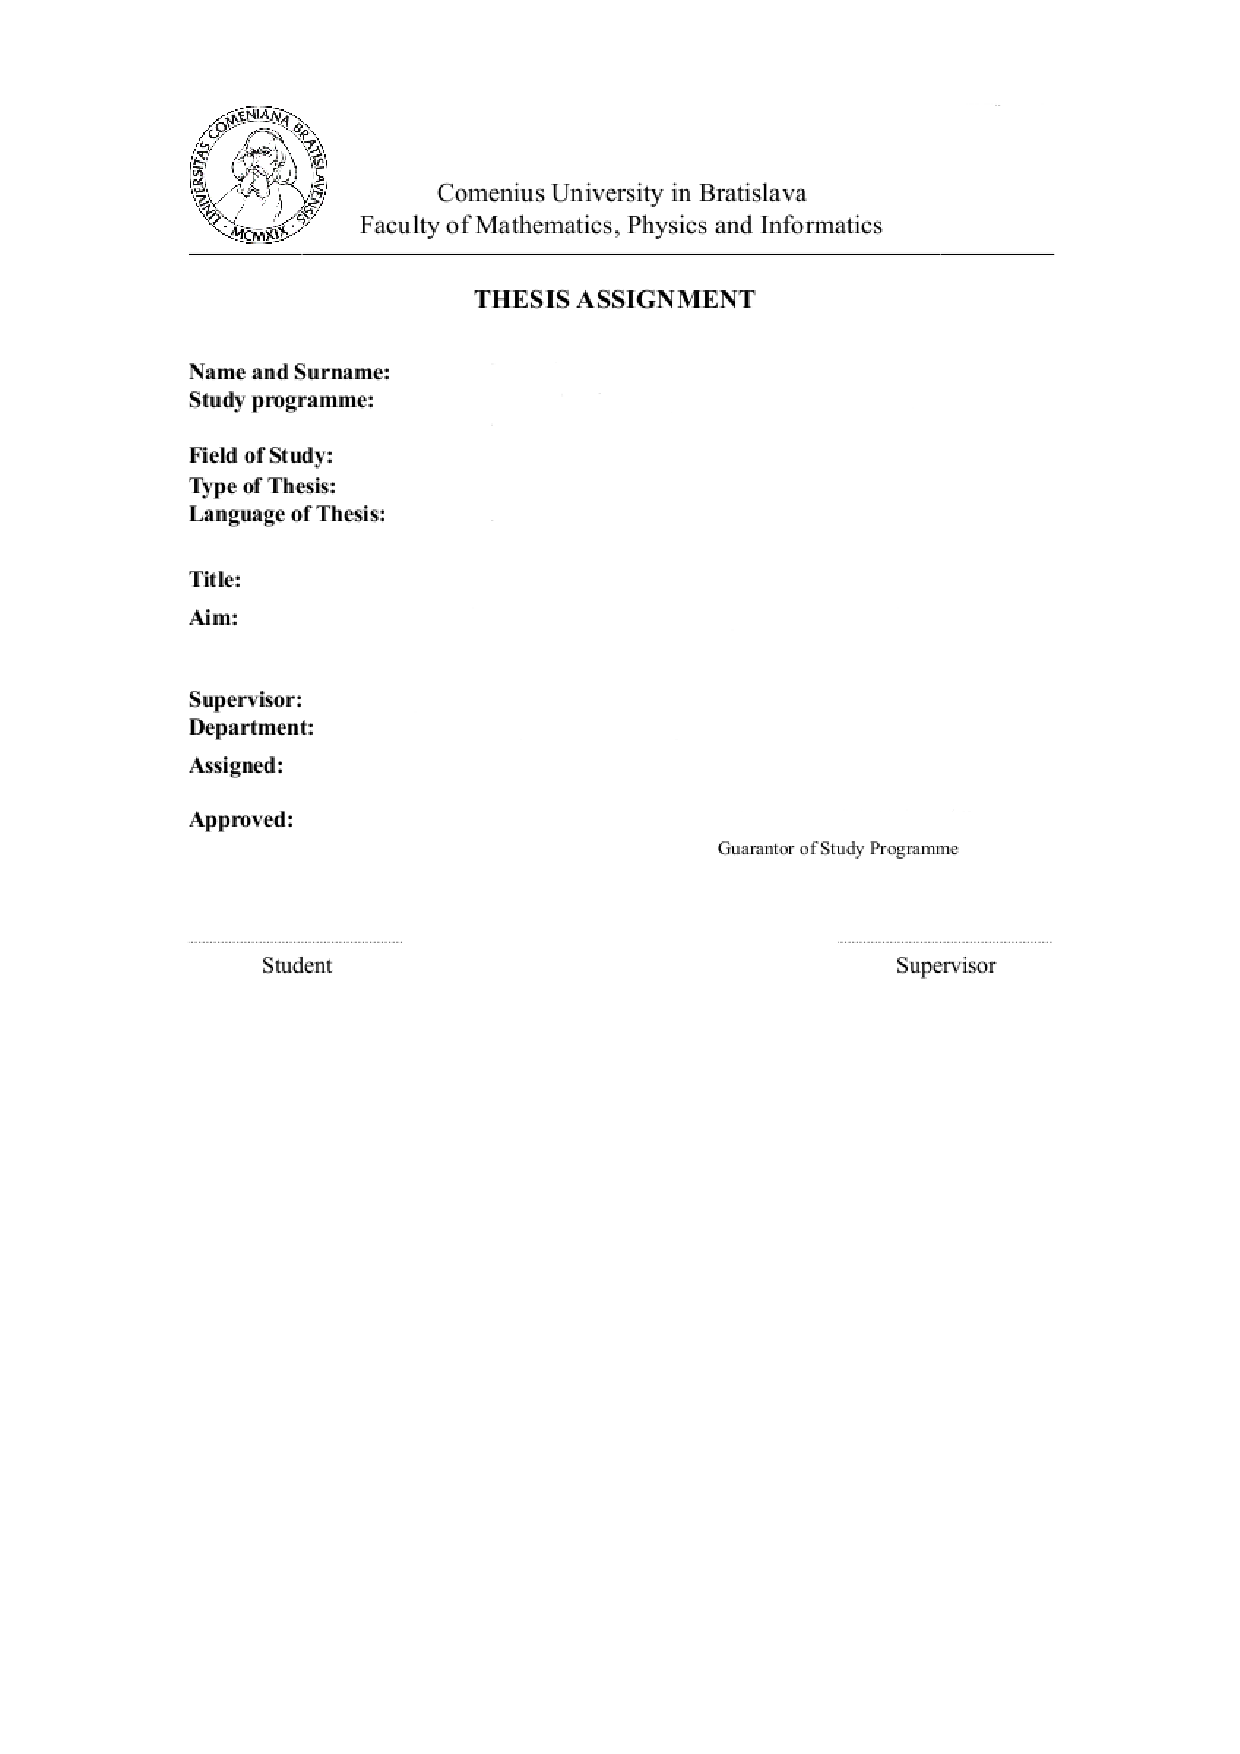
\includepdf[pages=-]{frontmatter/assignment.pdf}
%ZADANIE SK
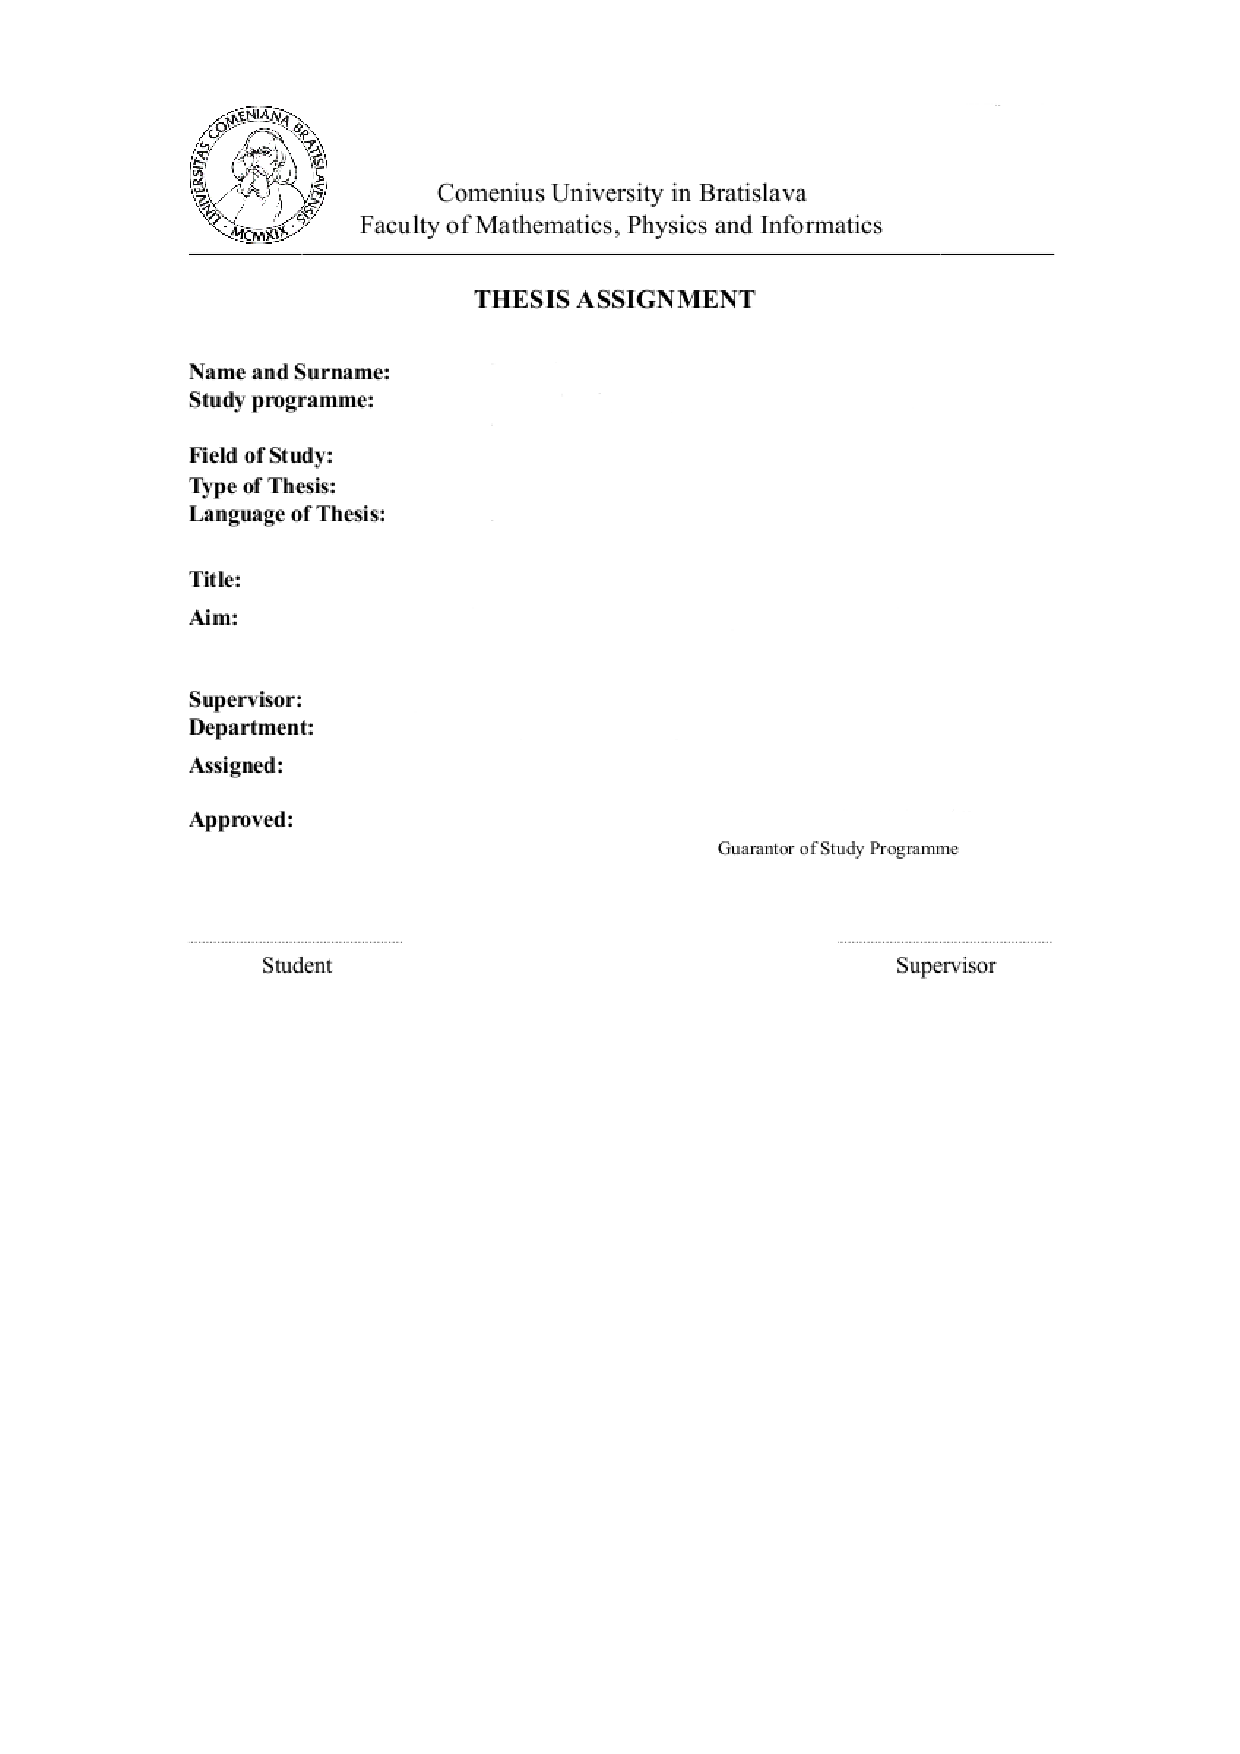
\includepdf[pages=-]{frontmatter/assignment.pdf}
\shorthandon{-}

%PODAKOVANIE
\chapter{Acknowledgement}
\vfil
\vfil
\vfil
\vfil
I would like to thank my supervisor \supervisor for his help and advices.


%ABSTRAKT EN
\chapter{Abstract}
We have implemented a method, that generates base manifold mesh from an input skeleton, based on Skeleton to Quad Dominant Mesh (SQM) algorithm, which converts skeletons to meshes composed mainly from quadrilaterals.
Each node in skeleton has assigned a sphere.
SQM algorithm first creates branch node polyhedrons for each sphere corresponding to a branch node.
These polyhedrons are bridged with quadrilaterals to create the final base mesh.
We have extended the algorithm to support generation of meshes from cyclic skeletons.
We have also generalized skeleton nodes to ellipsoids instead of spheres.
Finally, we extended the algorithm to generate meshes from linear skeletons without branching and from skeletons, which root node is not a branch node.
The generated base mesh is tessellated on GPU for better visual results.
\\ \\
\textbf{\textsc{Keywords:}} skeleton, convert, base mesh, manifold


%ABSTRAKT SK
\selectlanguage{slovak}
\chapter{Abstrakt}
V tejto práci navrhujeme algortimus, ktorý generuje základné manifoldné meshe zo vstupnej kostry, založený na algoritme Skeleton to Quad Dominant Mesh (SQM), ktorý konvertuje kostry na meshe zložené prevažne zo štvoruholníkov.
Každý vrchol kostry má priradenú guľu.
Algoritmus SQM najprv pre každý vrchol v ktorom sa kostra vetví vygeneruje polyhedrón, aproximujúci guľu príslušného vetviaceho sa vrcholu.
Neskôr sú tieto polyhedróny spojené štvoruholními, čím sa vytvorí základný mesh.
Rozšírili sme SQM algoritmus tak, aby generoval základné meshe aj z cyklických kostier.
Tiež sme zovšeobecnili vstupnú kostru tak, aby bolo možné zadávať elipsoidy namiesto gulí pre každý vrchol.
Nakoniec sme rozšírili algoritmus tak aby vedel generovat základné meshe aj z lineárnych kostier a z kostier, ktorých koreň nie je vetviaci sa uzol.
Vygenerovaný základny mesh teselujeme na grafickej karte, aby sme dosiahli lepsie vizuálne výsledky.
\\ \\
\textbf{\textsc{Kľúčové slová:}} kostra, konverzia, manifold, zakladný mesh

%PREDHOVOR
\selectlanguage{english}
\chapter{Preamble}
\paragraph{}
Lorem ipsum dolor sit amet, consectetur adipiscing elit. Nunc tristique, sem et feugiat ornare, lorem eros mattis odio, et tempus lectus ipsum nec ante. Phasellus interdum nunc ut sapien semper porttitor. Nam mi erat, faucibus in fermentum eu, varius eu velit. Integer egestas iaculis varius. In pulvinar, ligula eget adipiscing suscipit, nisl ipsum aliquet arcu, eget tristique felis leo vitae magna. Nulla et magna sed justo accumsan ultrices a in leo. Suspendisse tincidunt malesuada leo, eget rhoncus ipsum fringilla at. Integer et tortor vitae nisl fermentum vestibulum. Fusce eu dui neque, a egestas nunc. Vivamus condimentum mi non arcu lacinia et aliquam risus euismod. Nunc ut risus nec elit luctus aliquet et sit amet magna. Vestibulum vehicula enim eget erat fermentum a lacinia purus varius.

\paragraph{}
Duis tempus sem sit amet elit accumsan ultricies. Curabitur a nibh ante, vitae pharetra nulla. Suspendisse non risus elit, in aliquam felis. Maecenas suscipit placerat commodo. Vivamus et molestie odio. Quisque ut augue mi. Quisque aliquam luctus est, ac dignissim ante adipiscing eget. Quisque volutpat, sem vitae placerat condimentum, nunc lorem malesuada leo, sit amet pretium nisi felis nec lorem. Pellentesque nisi ipsum, vestibulum sed lacinia sed, condimentum a turpis.

\paragraph{}
In posuere convallis lectus vel hendrerit. Cras suscipit mi risus. Cum sociis natoque penatibus et magnis dis parturient montes, nascetur ridiculus mus. Donec ante nunc, cursus ac vulputate at, bibendum eget nisi. Nunc eget nunc sed massa blandit posuere id vel quam. Duis bibendum orci vel ligula tempor condimentum. Nulla pharetra tortor at risus dignissim fringilla. Nullam ac massa et nibh auctor vestibulum quis vitae ligula. Suspendisse ultrices eros sit amet lectus dictum dapibus. Sed congue, turpis nec aliquam fermentum, diam nisi cursus nibh, id vulputate massa tellus sit amet turpis.


%OBSAH
\tableofcontents

%ZOZNAM ILUSTRACII
\listoffigures

%ZOZNAM TABULIEK
\listoftables


\mainmatter
\chapter*{Introduction}
\addcontentsline{toc}{chapter}{Introduction}

Skeletal structures are often used in computer graphics to represent basic topology of a model.
This representation allows artists to conveniently animate articulated models, by manipulating key points represented as nodes in skeletons.
Skeletons corresponding to a model, are often provided by an artist, or extracted directly from a model \cite{laplac}.
Since skeletal structures carry information about the topology of a model, we could apply a reverse process to skeleton extraction and recover the base mesh represented by a skeleton.

Such base meshes, generated directly from skeletal structures, could be used to ease the modeling of base models of articulated characters.
An artist would only design the skeleton of the model and the base mesh would be generated automatically.

This technique can also be used to procedurally generate articulated models.
A skeleton can be either procedurally generated or manually entered.
A base mesh generated from a supplied skeleton can be augmented with procedurally generated displacement maps in order to generate a complex model.

In this thesis we will start with presenting the state of the art algorithms in the field of generating base meshes from skeletal structures.
We will analyze each proposed solution and pick the one best suited for our needs as base of our own algorithm.
Next, we will describe how we implemented the selected base algorithm as well as how we implemented our proposed extensions to the algorithm.
In the following chapter, we will present implementation details of our system, used programming language, libraries and design patterns.
In the last two chapters, we will present results of our work and summarize our goals in conclusion.

\pagebreak

\section*{Goals}
\addcontentsline{toc}{section}{Goals}

The goal of this thesis is to implement an algorithm that would be able to generate base manifold meshes corresponding to input skeletons.
The algorithm should be able to handle various types of input skeletons such as cyclic skeletons and linear skeletons, without branching.
The generated base mesh should be quad dominant.
Good edge flow of the generated base mesh is desired.
That means faces of the generated base meshes should be aligned with bones of their corresponding input skeleton.
The generated base meshes should have an option to terminate leaf nodes as capsules.
The algorithm should not be iterative and should not have any input parameters.
This way it could be used in interactive or fully automatic systems.
GPU computation capability should be leveraged wherever possible to increase the speed of base mesh generation.

\chapter{Related Work}
\paragraph{}
Generating base meshes from skeletons aids in modelling and rigging of more complex meshes. The most notable algorithms are B-Mesh\cite{ji_bm} by Ji et al. and Skeleton to Quad Dominant Mesh\cite{sqm} (SQM) by J. A. Bærentzen et al. This algorithms are capable of generating quad-dominant manifold meshes with good edge flow. Generated meshes are convenient because thanks to quad dominance and good edge flow they are easily skinned. Since the mesh is generated from skeleton we also implicitly know how much each bone affects vertices of the mesh during animation. We will also discuss some results from Michal Mc Donells master thesis Skeleton-based and interactive 3D modelling\cite{sqm_phd}. In particular the generation of capsule endings in SQM algorithm as we also wanted our algorithm to be capable of generating capsules.
\paragraph{}
B-Mesh algorithm and SQM algorithm present two different approaches to generation of base meshes from skeletons. B-Mesh algorithm firstly generates mesh for the limbs of the skeletons. These limb meshes are later joined together. On the other SQM algorithm firstly creates polyhedrons for branch nodes of the input skeleton. These polyhedrons are later joined with tubes consisting solely from quadrilaterals.
\paragraph{}
In this chapter we will describe both algorithms with their advantages and disadvantages. This serves to show why we have based our implementation on SQM algorithm.
\pagebreak

\section{B-Mesh algorithm}
\paragraph{Input}
B-Mesh algorithm takes as input a skeleton with a set of spheres or ellipsoids. Each node of the input skeleton has assigned a sphere or ellipsoid that represents its local geometry. Auxiliary spheres can be added to more precisely affect the resulting geometry of generated base mesh.
\paragraph{}
The algorithm consist of five steps:
\begin{enumerate}[\bfseries {Step} 1{:}]
	\itemsep-0.25em 
	\item Sphere generation - new spheres are generated along the bones of the skeleton.
	\item Sweeping - generation of mesh for skeletons limbs.
	\item Stitching - joining of limb meshes at branch nodes.
	\item B-Mesh evolution - subdivision and smoothing of generated mesh.
	\item B-Mesh fairing - fairing to improve edges flow.
\end{enumerate}
\begin{figure}[h]
    \centering
    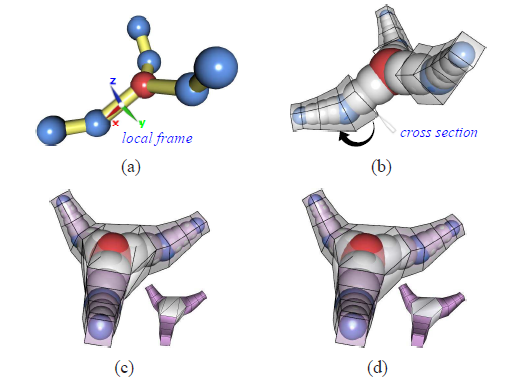
\includegraphics{images/b_mesh_ilu.png}
    \label{fig:b_mesh_stitch}
    \caption[B-Mesh sweeping and stitching illustration]{B-Mesh sweeping and stitching illustration. (a) local coordinates of a bone; (b) sweeping step; (c) stitching step; (d) after stitching simplification; Source \cite{ji_bm}}
\end{figure}

%\subsection{Sphere generation}
%\paragraph{}
\paragraph{Sphere generation}
Additional spheres are generated along the bones of the input skeleton. The distance between two spheres is defined by sampling step and the radius of each sphere is interpolated from radius's corresponding to the bones nodes. These generated spheres are used to refine the generated mesh and to calculate scalar field need in B-Mesh fairing step.

%\subsection{Sweeping}
%\paragraph{}
\paragraph{Sweeping}
For each bone its local coordinate system is generated as can be seen in Figure \ref{fig:b_mesh_stitch} (a). Limb mesh generation starts at branch nodes. For each new limb a rectangle aligned with limbs corresponding bones local axis is generated. Its points are then translated along the bones forming said limb and rotated around the connection nodes. After each translation the new points are connected with previous set of points in order to form a tube consisting of quadrilaterals. The resulting tubes can be seen in Figure \ref{fig:b_mesh_stitch} (b).

%\subsection{Stitching}
%\paragraph{}
\paragraph{Stitching}
Limb meshes generated in sweeping step are now stitched together. This is done by generating a convex hull from all the points corresponding to each branch nodes. These points are the beginning of each limb mesh tube. The result can be seen in Figure \ref{fig:b_mesh_stitch} (c). Generated convex hull is composed from triangles. To simplify them into quadrilaterals a score between each pair of triangles is computed. The score measures how close to a plane is each pair of triangles. The results of stitching simplification are shown in Figure \ref{fig:b_mesh_stitch} (d).

\paragraph{B-Mesh evolution}
Catmull-Clark subdivision is used to smooth the stitched mesh. However after smoothing the mesh shrinks and deviates from the spheres. A scalar field is generated and used to evolve the mesh. Each vertex of the stitched mesh is translated according to the scalar field and its evolution speed. This means the further away is the vertex from its corresponding sphere the more it is attracted to it. In this phase the auxiliary spheres are used to manipulate the scalar field and thus the final shape of the mesh. This step can be repeated multiple times to further smooth the mesh.

\paragraph{B-Mesh fairing}
After the evolution step certain edges may not be aligned with their principal directions. New vertex positions are calculated by iterative minimization of a function.

\paragraph{Conclusion}
The biggest problem with B-Mesh algorithm for our use is its iterative nature. The number of iterations is an input parameter and we wanted to avoid input parameters, so that the base mesh generation is as automatic as possible. Without the evolution step B-Mesh approximates input geometry worse than SQM. This is caused by the stitching phase which creates rectangular geometry at branch nodes, instead of the input spherical or elliptical geometry. Because of this evolution phase can not be avoided if we want to approximate the input as much as possible.
\paragraph{}
B-Mesh algorithm is also running slower and produces more triangles than SQM according to \cite{sqm}. The auxiliary spheres and ellipsoid nodes are interesting additions that were not present in SQM. But we wanted to modify the generated base mesh geometry directly on GPU during rendering so they are not advantageous to our intended use. B-mesh algorithm can generate capsules but it needs several evolution steps to precisely match capsules geometry. The algorithm looks like it can be naturally extended to support cyclic skeletons. Sweeping steps occurs only on limb paths and stitching occurs directly at branch nodes. Evolution and fairing moves vertices directly so it is independent from cycles in the input skeleton.

\section{Skeleton to Quad Dominant Mesh algorithm}
\paragraph{Input}
The input to SQM algorithm is a skeleton. Similarly to B-mesh for each of skeletons nodes a sphere is defined to represent local geometry. Contrary to B-mesh algorithm SQM does not support ellipsoid nodes. SQM algorithm has also an extra limitation that the root of the skeleton has to be a branch node.
\paragraph{}
The algorithm consist of four steps and one preprocessing step:\\
\textbf{Preprocessing:} Skeleton straightening - serves to simplify step number 3 of the algorithm.
\begin{enumerate}[\bfseries {Step} 1{:}]
	\itemsep-0.25em 
	\item BNP generation - generation of branch node polyhedrons (BNPs).
	\item BNP refinement - subdivisions of BNPs.
	\item Creating the tubular structure - bridging of BNPs.
	\item Vertex placement - reverting straightened mesh to its original pose.
\end{enumerate}

\begin{figure}[h]
    \centering
    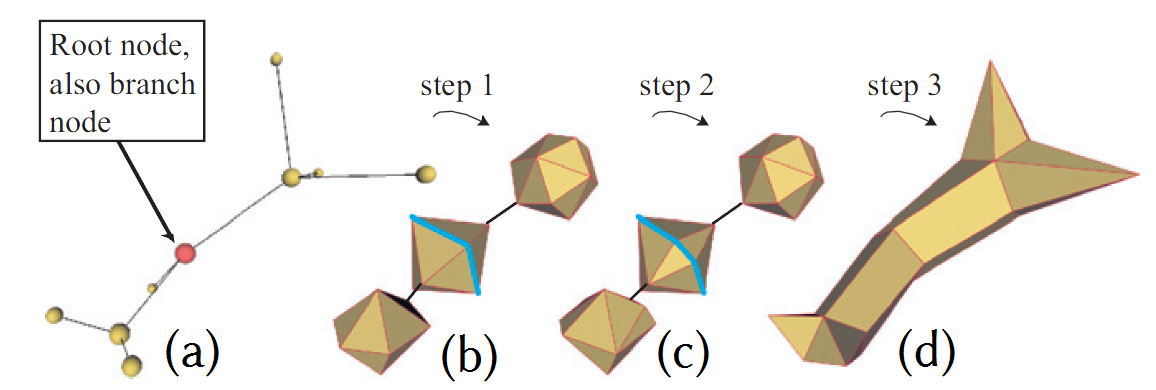
\includegraphics[width=\textwidth]{images/sqm_viz.png}
    \label{fig:sqm_algorithm_steps}
    \caption[Steps of SQM algorithm]{Steps of SQM algorithm. (a) the input skeleton; (b) generated BNPs; (c) refined BNPs; (d) BNPs bridges with quadrilateral tubes; Source \cite{sqm}}
\end{figure}

\paragraph{Skeleton straightening}
This is a preprocessing step of the algorithm that simplifies the generation of tubular structures. For each connection node its child is rotated, so that the edge between connection node and its child is parallel with the edge between connection node and its parent. This is usefully because during step 3 the algorithm needs to only generate straight tubes and does not need to take rotation into account.

\paragraph{BNP generation}
A branch node polyhedron(BNP) is a polyhedron assigned to a branch node. Vertices of a BNP correspond to a set of points that are generated by intersecting the sphere assigned to a branch node with each edge connected to said branch node. We will call this vertices intersection vertices. To form a BNP intersection vertices are triangulated. After that each triangle is split into six triangles by inserting one vertex in the middle of each triangle and in the middle of each of the edges of the triangle. These vertices are then projected back onto the sphere associated with a branch node. This projection is needed because if the intersection vertices are coplanar the generated polyhedron would have no volume. The result of this step can be seen in Figure \ref{fig:sqm_algorithm_steps} (b).

\paragraph{BNP refinement}
During step 3 of the algorithm BNPs connected via path are bridged with tubes consisting solely from quadrilaterals. This is done be connecting the one-rings of two corresponding intersection nodes with faces. To ensure that we can use only quadrilaterals the one-rings need to have the same valency. So each BNP is refined so that the valency of two intersection nodes lying on the same path are equal. This can be seen in Figure \ref{fig:sqm_algorithm_steps} (c).

\paragraph{Creating the tubular structure}
After previous step of the algorithm connected BNPs can be joined by a tube formed by quadrilaterals. The tube is divided into segments. Each of the segments corresponds to a connection node. Vertices corresponding to a certain connection node are projected onto its corresponding sphere. Leaf nodes are terminated with a triangle which central vertex corresponds to the leaf nodes vertex. The result is illustrated in Figure \ref{fig:sqm_algorithm_steps} (d).

\paragraph{Vertex placement}
The base mesh is now finished. All that remains is to reverse the rotations used to straighten the input skeleton. After final vertex placement the resulting mesh is smoothed using with three iterations of Laplacian smoothing and attraction scheme.

\paragraph{Conclusion}
Each of SQMs steps are one pass algorithms except the final smoothing and attraction scheme application. But since SQM generates branch node geometry by generating a polyhedron it better resembles the geometry of the input skeleton even without smoothing. Cyclic meshes can be problematic to implement, because in the refinement step of the algorithm a cyclic mesh may cause an infinite loop of refining.

\paragraph{}
In the end we have picked SQM as the base for our algorithm. The main factors in this decision were that SQM is faster, produces smaller number of triangles and even without smoothing the generated mesh better resembles the input skeleton. Also by avoiding the smoothing phase we don not need any input parameters to generate base mesh from an input skeleton.

\section{Skeleton-based and interactive 3D modelling} 
\paragraph{}
Michal Mc Donells master thesis studies the capabilities of SQM algorithm. It aims to extend SQM algorithm through pre-processing of SQMs input skeleton and post-processing of the output mesh. Altering SQM algorithm itself was out of scope of the thesis. Among the improvements to the algorithm were cone, cube, sphere and hemisphere leaf nodes, cube connection and branch nodes as well as concavities and branch node root requirement. The most important parts for us are spherical leaf nodes and branch node root requirement.

\begin{figure}[h]
    \centering
    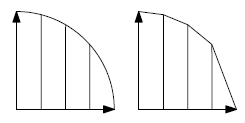
\includegraphics[]{images/spherical_node.png}
    \label{fig:esqm_spherical}
    \caption[Spherical nodes radii]{Left: arc subdivided at fixed intervals; Right: radii of newly inserted nodes sampled from an arc on the left; Source \cite{sqm_phd}}
\end{figure}

\paragraph{Spherical leaf node}
Original SQM algorithm was not able to create spheres at leaf nodes. This also limited its ability to generate capsules that we wanted to implement in our algorithm. In the thesis a solution was presented that a spherical node would be represented by several connection nodes. The first connection node would have the same radius as the desired sphere and each subsequent node would have its radius decreased until the desired number of subdivisions would be reached. We can see the process in Figure \ref{fig:esqm_spherical}. An arc with equal radius as the original spherical node would be sampled at fixed intervals. With enough samples the resulting mesh would approximate a sphere. However in the original SQM algorithm after Laplacian smoothing the smoothed mesh did not approximate the input sphere.

\paragraph{Conclusion}
The approach to create spherical nodes presented in the thesis seems suitable for our needs. Since we would not implement Laplacian smoothing we would not have problems with deformation of the generated sphere. On the contrary this approach is beneficial to our needs, since we wanted to smooth the generated mesh in tessellation shaders and keeping spherical meshes generated without post-processing can potentially ease the work-flow.

\paragraph{Root branch node requirement}
One of the limitations of SQM algorithm is that the root node has to be a branch node. The proposed solution to this limitation was to generate pseudo paths from the root to ensure that it always will have at least three child nodes. For example, if the root has only two childes the new node would be generated in a direction perpendicular to a line connecting the intersection of roots associated sphere and edges from root to its childes.

\paragraph{Conclusion}
This pseudo path generation would disturb the edge flow as it would introduce new unnecessary edges. We believe that a better approach would be to re-root the tree and replace its former root with a node with at least three childes. Linear skeletons without branching and skeletons consisting only from a single node would become special cases that would be handled separately. This would allow us to avoid the requirement without altering the expected edge flow of the input skeleton.

\chapter{Proposed solution}\label{ch:proposed_solution}
\paragraph{}
We have picked SQM as the base for our algorithm. The main factors in this decision were that SQM is faster, produces smaller number of triangles, has better edge flow and even without smoothing the generated mesh better resembles the input skeleton. By avoiding the smoothing phase we do not need any input parameters to generate base mesh from an input skeleton. In this chapter we will explain each step of our proposed algorithm as well as extensions like elliptical nodes, cycles, etc.

\section{Skeleton straightening}\label{sec:straight}
Skeleton straightening is a preprocessing step that simplifies bridging of branch node polyhedrons. Straightened skeleton is a skeleton which nodes in every path between two branch nodes, two leaf nodes, or a branch node and a leaf node are co-linear. In addition we have added an extra condition that angles between child nodes of a branch node should be the same in straightened skeleton as they are in the input skeleton. To achieve the first condition for each connection node, we take the direction of a vector formed by connection nodes parents’ position and connection nodes position. The direction vector can be seen in Figure \ref{fig:straightening_ilu} as the green arrow. Then we normalize the direction vector and multiply it by the distance between connection node and its child node. The distance is marked by the black curve in Figure \ref{fig:straightening_ilu}. This vector represents the offset form connection nodes position at which lies the straightened position of its child node. We then calculate rotation between connection nodes child original position and its new position, in respect to the position of connection node. Finally, we rotate all descendants of the connection node. In order to conform to the second condition, at each branch node we do not alter the position of its child nodes.

\begin{figure}[h]
    \centering
    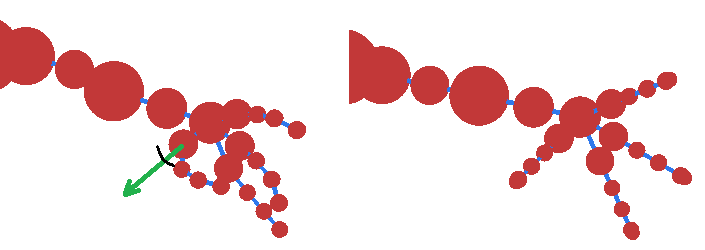
\includegraphics[width=\textwidth]{images/straightening2.png}
    \caption[Skeleton straightening]{Skeleton straightening. Left: input skeleton, green arrow represents the direction from connection nodes parents position to connection nodes position, black curve marks the distance between connection node and its child; right: straightened skeleton.}
    \label{fig:straightening_ilu}
\end{figure}

\subsection{Skinning}
In final vertex placement, we need to undo the rotations applied to the input skeleton during straightening. We have decided that the best solution is to use skinning since it can be implemented on GPU and we wanted to move all post-processing on the GPU. Straightened skeleton represents bind pose for skinning purposes and the input skeleton represents reference pose. Now we can calculate rotations, represented as quaternions, required to transform bind pose to reference pose. Traditionally, this would require to find the rotation between two corresponding nodes in respect to their parent. Rotating all child nodes in bind skeleton using the same rotation and propagate the rotation calculation to child nodes. However, since we know precisely how bind pose was constructed, we can exploit this knowledge and avoid the rotation of child nodes.
In fact, we do not even need the bind skeleton itself because the positions can be calculated from reference pose.

We want to calculate the rotation that would transform a node from its bind pose to its reference pose.
We know that the nodes parent is already in reference pose.
We also know that bind pose was constructed in such a way that all connection nodes child nodes are co-linear and preserve the distances between nodes.
That means from nodes parent reference pose we can calculate where would the node be in bind pose, if we would apply on it the same transformation matrices as were applied to its parent node.
The distance between parent and child nodes remains constant in both poses. And the direction at which the child node would be in bind pose is the same as the direction from its grandparent node to its parent node.
Now we only need to store the rotation between calculated child node position in bind pose and its actual position in reference pose with respect to its parent node.
The following algorithm demonstrates the calculation of a quaternion required to transform one node from straightened bind pose to input reference pose:
\begin{align*}
node& \leftarrow nodeInReferencePose \\
parent& = node.Parent \\
grandParent& = parent.parent \\
distance& = dist(node, parent) \\
direction& = normalize(parent - grandParent) \\
nodeInBind& = parent + distance * direction \\
u& = normalize(nodeInBind - parent) \\
v& = normalize(node - parent) \\
rotation& = QuaternionBetweenVectors(u, v)
\end{align*}



%In fact we do not even need the bind skeleton itself.
%
%This can be seen in Figure \ref{fig:DoF_estimation_ilu}. We want to calculate the rotation that would transform circle node to reference pose. We know that circle nodes parent square node is already in reference pose. We also know, that bind pose was constructed in such a way that all connection nodes childes are co-linear and preserve the distances between nodes. That means from squares reference pose we can calculate, where would be circle node, if we would apply on it the same transformation matrices as were applied to square node. The distance between square and circle node remains constant in both poses. And the direction at which the circle node would be is the same as the direction from triangle node to square node, which is marked as green arrow in Figure \ref{fig:DoF_estimation_ilu}. Now we only need to store the rotation between calculated circle node position, green circle in Figure \ref{fig:DoF_estimation_ilu} and its actual position red circle, with respect to its parent red square node.
%
%\begin{figure}[h]
%    \centering
%    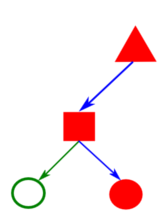
\includegraphics[height=6cm]{images/DoF_estimation.png}
%    \label{fig:DoF_estimation_ilu}
%    \caption[Rotation estimation from reference pose]{Rotation estimation from reference pose. Circle: node which rotation we want to estimate; Square: parent of circle node; Triangle: parent of square node; Blue arrows: edges in reference pose; Green circle: circle node position after applying squares skinning matrices; Green arrow: direction from square to green circle node;}
%\end{figure}

\section{BNP generation}\label{sec:bnp_gen}
For each branch node we calculate the direction from said branch node to each of its children and to its parent. Then we create rays with origin in branch nodes position and direction corresponding to the direction calculated previously. These rays can be seen in Figure \ref{fig:bnp_gen_ilu}a as blue arrows. We calculate the intersection of each of these rays with the sphere associated with the branch node. We store each intersection in a set of intersection points. Now we triangulate the intersection points. Different algorithms can be used to achieve the same effect, but we have picked Delaunay triangulation in spherical domain which was also used in the original paper. The algorithm works like standard Delaunay triangulation. With one exception, the predicate deciding whatever newly inserted triangle would lay in the circle of an already existing triangle is replaced. The new predicate compares angle between the newly inserted triangles normal with normals of already existing triangles. Result of triangulation is shown in Figure \ref{fig:bnp_gen_ilu}b as the blue triangle. We will use indexed face representation of the mesh, since that is the output of Delaunay triangulation. The generated polyhedron is now subdivided by inserting a point in the center of each face and in the middle of each edge. The vertex inserted in the center of each face is then connected with all vertices corresponding to the same face. So each triangle is subdivided into six smaller triangles. The newly inserted points are then projected onto the sphere associated with the node. The subdivision and projection is necessary because otherwise polyhedrons that would be generated with co-planar or nearly co-planar intersection points would have zero volume or very small volume, respectively. To project the newly inserted vertices onto the sphere, we once again use a ray-sphere intersection. The origin of the ray is the position of each newly inserted vertex. The direction of the ray is mean normal of the faces that are connected with the vertex. This means that for the vertices in the center of each face the normal of the subdivided face is used. For vertices inserted in the middle of each edge the mean normal of faces corresponding to that edge is used. Final polyhedron is shown in Figure \ref{fig:bnp_gen_ilu}c.

\begin{figure}[h]
    \centering
    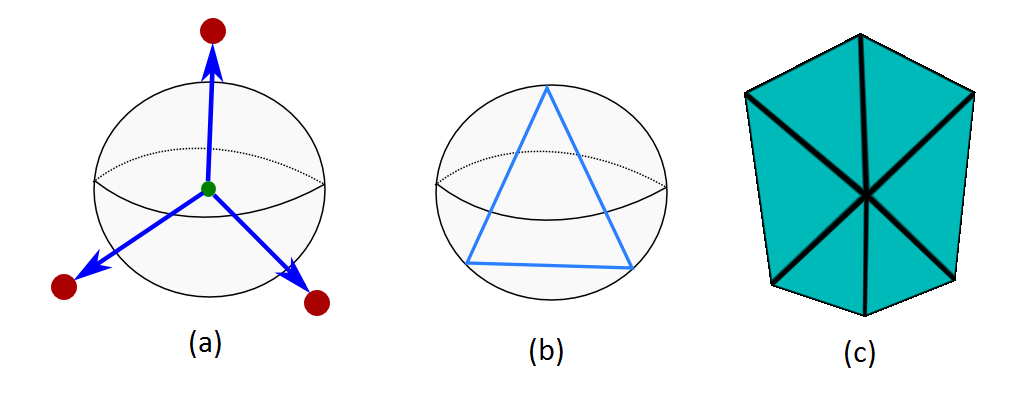
\includegraphics[width=\textwidth]{images/bnp_gen_ilu.png}
    \caption[BNP generation process]{BNP generation process. (a) green is a branch node, blue arrows represent direction vectors of rays, red circles represent child nodes; (b) blue triangle is the result of triangulation; (c) final subdivided BNP.}
    \label{fig:bnp_gen_ilu}
\end{figure}

Triangulation of intersection vertices can sometimes create obtuse triangles. These are problematic because when we insert the vertex in the middle of an obtuse triangle the one-rings of intersection vertices are not convex. If we would project the one-ring of the intersection vertex onto a plane, which is defined by the intersection point and the direction from skeletal nodes position to the intersection point, the resulting planar polygon would not be convex. In Figure \ref{fig:obtus_tri_ilu} we can see on the left how a polyhedron looks when it is generated with obtuse triangles. Expected central vertex position is marked by red arrow and expected edges are marked as yellow lines. This is not desirable since it would cause problems during cyclic mesh generation. To remedy this situation we calculate the projection of the central vertex in a different manner. The origin of the ray is the position of the vertex. But we use a new direction vector. This vector is the normal of a triangle formed by the projected points that were inserted in the middle of each edge. The result can be seen in Figure \ref{fig:obtus_tri_ilu} on the right.

\begin{figure}[h]
    \centering
    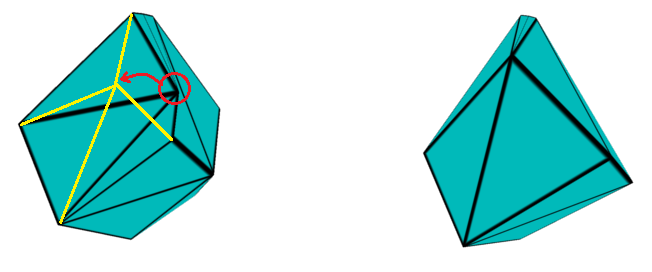
\includegraphics[height=4cm]{images/obtuse_triangle_fix_ilu.png}
    \caption[Obtuse triangle problem]{Obtuse triangle problem. Left: polyhedron with obtuse triangle. Red arrow marks vertex expected position and yellow lines mark expected edges; right: polyhedron after applying our fix.}
    \label{fig:obtus_tri_ilu}
\end{figure}

\section{BNP refinement}\label{sec:bnp_sub}
During the penultimate step of the algorithm, BNP joining, we want to connect two BNPs, with tube consisting solely from quadrilaterals. To ensure that we can use quadrilaterals only, we want intersection vertices connected via a path, to have the same number of nodes in their one-ring neighborhood. We take the notion of Link Intersection Edge (LIE) from \cite{sqm}. A LIE is a set of edges that are between vertices of two intersection vertices one-ring neighborhoods. In Figure \ref{fig:refinement_ilu}a one LIE is represented with yellow colored edges and a second LIE is represented with red colored edges. The refining of one BNP is a one-pass procedure. Since we will often need to access the one-ring neighborhood of a vertex, we convert our mesh to half-edge representation.

\paragraph{Preprocessing}
We start the refining of a BNP by creating a map of LIEs corresponding to each intersection vertex. For each intersection vertex, we store its corresponding LIEs, as well as the number of splits required by that vertex, to have the same valence as its corresponding vertex. An intersection vertex can be connected with three types of vertices. Each type defines how much we can split LIEs, corresponding to that intersection vertex.
\begin{itemize}
	\itemsep-0.25em 
	\item \textbf{Parents intersection vertex} - the number of splits is fixed. That is after splitting the valence of these two vertices must be exactly the same. This is necessary otherwise splits in child BNP could cause splits in parents BNP which could result in infinite loops.
	\item \textbf{Branch node intersection vertex} - difference between valencies of the two vertices is calculated. If the number is negative, that is corresponding vertex has smaller valence, we prefer not to split LIEs corresponding to current intersection vertex. If the number is positive, that is corresponding vertex has higher valence, we split LIEs corresponding to current intersection vertex so that the vertex has at least the same valence as its corresponding vertex.
	\item \textbf{Leaf node} - corresponding LIEs can be split as much as needed.
\end{itemize}

\begin{figure}[h]
    \centering
    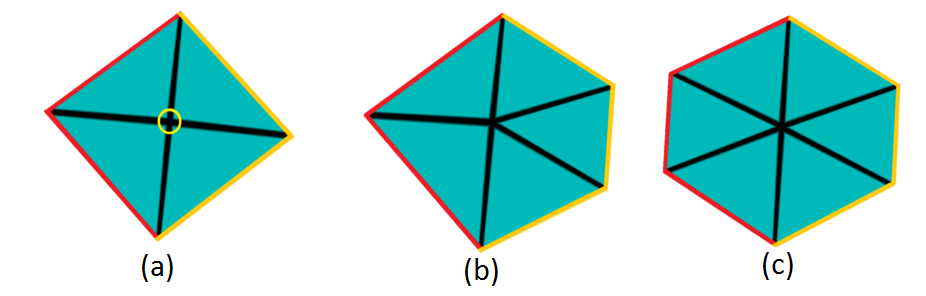
\includegraphics[width=\textwidth]{images/refinement_ilu.png}
    \caption[BNP refinement]{BNP refinement. Yellow edges represent Link Intersection Edge (LIE) corresponding to second intersection edge of the BNP. Red edges represent LIE corresponding to third intersection edge. Yellow circle marks the first intersection vertex. (a) BNP before subdivision; (b) BNP after one subdivision and one smoothing step; (c) final BNP after two subdivisions and two smoothing steps.}
    \label{fig:refinement_ilu}
\end{figure}

\paragraph{Subdivision}
We loop through all intersection vertices, starting with the intersection vertex connected with parents BNP and continuing with the rest. In each cycle, we split LIEs corresponding to current intersection vertex, until the valence of the intersection vertex is equal to its required number of splits. Every time we want to split a LIE we heuristically select the best based on two filters. The first filter is the splitting required by the other intersection vertex belonging to the same LIE. If two or more LIEs require the same number of splits we use a second filter. This filter picks the LIE that was split the least. When we are splitting a LIE, we always split a representative edge which is the first edge of the LIE. Because of that we need to apply a smoothing scheme to roughly equalize the lengths of edges in a LIE. 

The whole process can be seen in Figure \ref{fig:refinement_ilu}. In Figure \ref{fig:refinement_ilu}a the yellow circle marks an intersection vertex that needs to be split twice. Yellow edges represent a LIE corresponding to second intersection vertex and red edges represent a LIE corresponding to third intersection vertex. Both LIEs have the same need to be split and none of them was split previously. For the first split the yellow LIE is selected subdivided once and smoothed. The result of the first split is shown in Figure \ref{fig:refinement_ilu}b. For the second split the need of both LIEs is still the same. But yellow LIE was already split so this time the red LIE is selected, subdivided, and smoothed. Final refined BNP is shown in Figure \ref{fig:refinement_ilu}c.

\subsection{Smoothing}
Since we always split only one representative edge of a LIE we are applying a smoothing scheme to equalize the length of edges in a subdivided LIE. The smoothing is very important because generated base mesh quality directly depends on the selected smoothing scheme. Ideally, the length of each edge in a smoothed LIE would be equal. However, since smoothing is applied after every subdivision the smoothing algorithm should be reasonably fast. We propose four smoothing schemes. These smoothing schemes are illustrated in Figure \ref{fig:smoothing_ilu} where the polyhedron from Figure \ref{fig:refinement_ilu}a is subdivided twice and then smoothed with various smoothing schemes.

\paragraph{Averaging smoothing}
New position for each vertex on a LIE is calculated by averaging one-ring neighborhood corresponding to the vertex. We start with the last vertex of a LIE that is the vertex on the last edge of a LIE and move towards the first vertex. We move each vertex, except the first and the last vertices, to the barycenter of its one-ring neighborhood and project them back onto the sphere corresponding to BNPs node. The resulting smoothed polyhedron is shown in Figure \ref{fig:smoothing_ilu}a. This approach is iterative and would need several iteration to achieve global optimum. However, we have found that one iteration is enough for our needs.

\paragraph{Quaternion smoothing}
For each LIE we calculate a quaternion representing the rotation from the first vertex of the LIE to the last vertex of the LIE. From each quaternion we extract its corresponding axis of rotation and angle of rotation. We smooth only points between the first and the last vertex so the calculated axis of rotation and angle are constant. During each smoothing step we first count the number of vertices in a LIE. Then we divide the angle of rotation by that number and form a new quaternion from already calculated axis of rotation and the newly calculated angle. For each vertex in a LIE between first and last we apply the rotation stored in the quaternion and update its position. This method produces LIEs that lie on small circles of their corresponding sphere. The spacing between vertices is regular and thus its very suitable for our needs. The result of quaternion smoothing is shown in Figure \ref{fig:smoothing_ilu}b.

\paragraph{Area weighted Laplacian}
For Laplacian smoothing we have adapted the algorithm described in \cite{laplac}. The weights used for smoothing are based on the one-ring area of each vertex. We use one iteration of Laplacian smoothing and then project the new vertices back onto their corresponding sphere. The result is shown in Figure \ref{fig:smoothing_ilu}c. The result is usable since the edges have better distributed length, than without smoothing. However, averaging and quaternion smoothing produce results of better quality.

\begin{figure}[h]
    \centering
    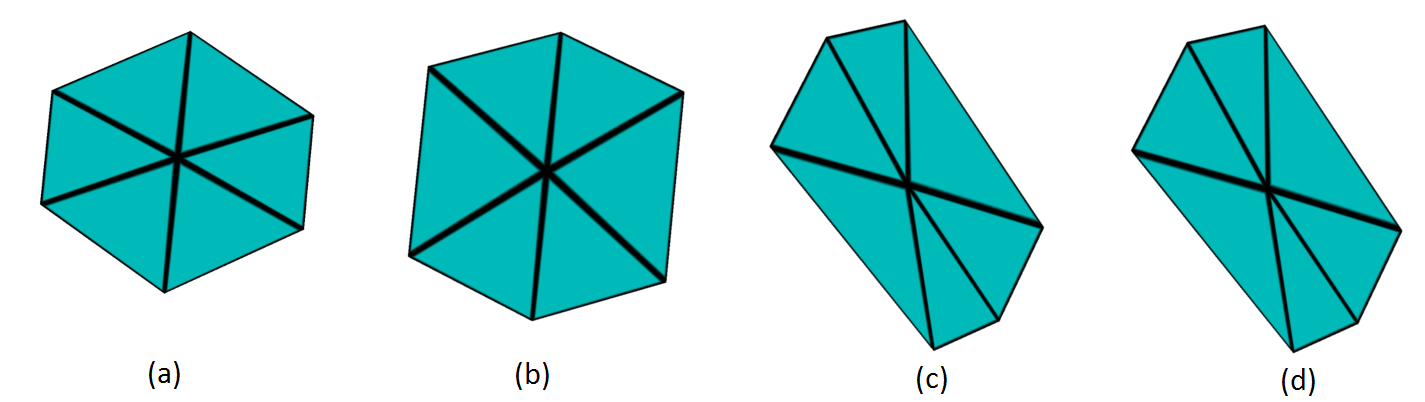
\includegraphics[width=\textwidth]{images/smoothing_ilu.png}
    \caption[LIE smoothing schemes]{LIE smoothing schemes. Shows results after applying: (a) averaging smoothing; (b) quaternion smoothing; (c) area weighted Laplacian smoothing; (d) valence weighted Laplacian smoothing.}
    \label{fig:smoothing_ilu}
\end{figure}

\paragraph{valence weighted Laplacian}
We use the same algorithm as for area weighted Laplacian with different contraction weights. The weights depend on the valence of each vertex. After Laplacian smoothing vertices are projected back onto their corresponding sphere. The result of this smoothing is very similar to area weighted Laplacian and is shown in Figure \ref{fig:smoothing_ilu}d.

\section{BNP joining}\label{sec:bnp_join}
After refinement of BNPs intersection vertices connected via path have the same valence. Now BNPs can be joined by tubes consisting from quadrilaterals only. We loop through each branch node in a depth-first search from skeletons root. We process each BNP in the following manner. We start with the whole BNP Figure \ref{fig:joining_process_ilu}a. We loop through all intersection vertices corresponding to current BNP. We remove each intersection vertex and its corresponding faces and edges from current BNP. In Figure \ref{fig:joining_process_ilu}b we can see the removal of third intersection vertex after first and second intersection vertices were joined. After the removal of an intersection vertex we continue joining all nodes on the path that produced the removed intersection vertex. We take the vertices forming the former one-ring of the removed intersection vertex. For each connection node on the path we duplicate the one-ring vertices, translate them to the nodes position and project them onto the sphere associated with the connection node. For the translation we construct a plane. The origin of the plane is the position of the connection node. The normal is the vector from the branch node to the connection node. Each vertex is translated along the normal until it lies on the plane. The projection is done by normalizing the vector from connection nodes position to each vertex and multiplying it by the radius of connection nodes corresponding sphere. These new vertices are then connected with previous set of vertices with faces and they are passed as current one-ring vertices for joining. In Figure \ref{fig:joining_process_ilu}c, we can see the translated connection node vertices before projection was applied. In Figure \ref{fig:joining_process_ilu}d the duplicated one-ring vertices are projected onto their associated sphere. After going through all connection nodes we can end either in a branch node or in a leaf node.

\begin{figure}[h]
    \centering
    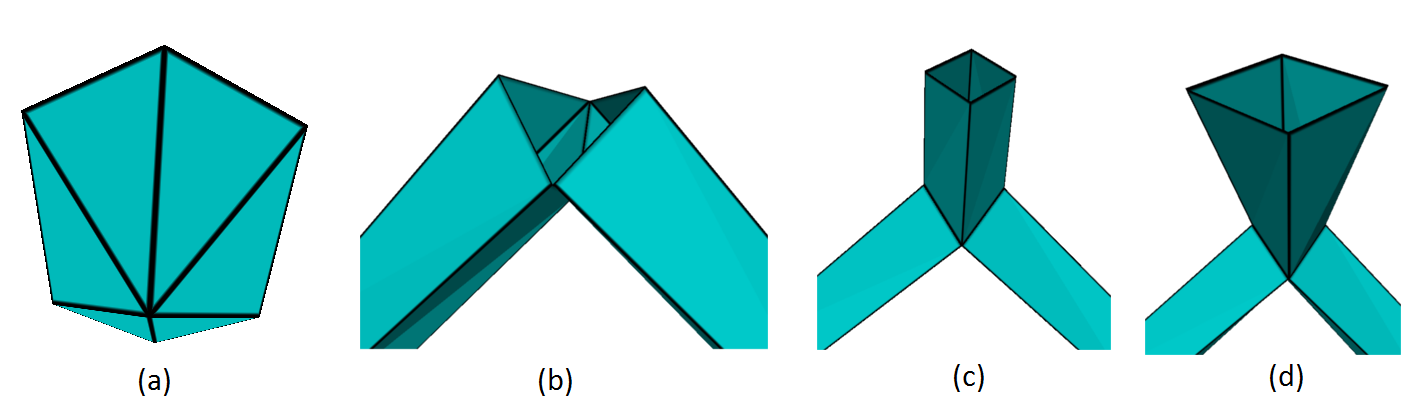
\includegraphics[width=\textwidth]{images/joining_ilu.png}
    \caption[BNP joining process]{BNP joining process. (a) polyhedron before joining; (b) polyhedron with removed faces corresponding to an intersection vertex; (c) new vertices for connection node before projection; (d) projected vertices of connection node.}
    \label{fig:joining_process_ilu}
\end{figure}

\paragraph{Branch node termination}
We start by removing the destination branch node corresponding intersection vertex and faces and edges connected to it. The tube generated from connection nodes should be joined with destination intersection vertex former one-ring. For this we need to find two corresponding vertices, which would form the first pair and define the pairing of the rest of the vertices. We can use multiple methods to find the first pair. The choice of the method affect output base mesh quality, as a wrong selection can lead into twists in the base mesh. We tested three methods.
\begin{itemize}
	\itemsep-0.25em 
	\item \textbf{Minimal Euclidean distance} - An arbitrary vertex is selected from current one-ring and its Euclidean distance to each vertex of destination one-ring is calculated. We match the vertex with the closest one. The main disadvantage of this method is that it is greedy end ends in local minima. That is to have the best overall mesh quality a more distant vertex would be a better choice. This can be seen in Figure \ref{fig:join_pairing_ilu}a where some connecting faces are twisted.
	\item \textbf{Minimal angle} - An arbitrary vertex is selected from the current one-ring. The direction from the selected vertex to each vertex of destination one-ring is calculated. Then we calculate the angle between this direction and the direction from original branch node to destination branch node. As a match we pick a vertex where the calculated angle was minimal. As before this method is greedy and can fall into local minima. An example of this is shown in Figure \ref{fig:join_pairing_ilu}b where some faces connecting the hand are twisted.
	\item \textbf{Minimal total Euclidean distance} - An arbitrary vertex is selected from current one-ring. We pair the vertex with each vertex of destination one-ring. Each pair defines a different mapping from the current one-ring vertices to destination one-ring vertices. We calculate the Euclidean distance between all paired vertices and store it as total Euclidean distance. Then we pick as pair the vertex where the total distance was minimal. The disadvantage of this approach is that it takes longer to compute. The advantage is that this approach avoids local minima by testing all the possible solutions and picking the best one. Since one-rings usually consist of few vertices we have decided to use this method. The resulting mesh using this pairing is shown in Figure \ref{fig:join_pairing_ilu}c. Among the possible results in Figure \ref{fig:join_pairing_ilu}c has minimal twisting compared to Figure \ref{fig:join_pairing_ilu}a and Figure \ref{fig:join_pairing_ilu}b. 
\end{itemize}

When the pairing of vertices is defined new edges can be formed between each pair and connect the geometry.

\begin{figure}[h]
    \centering
    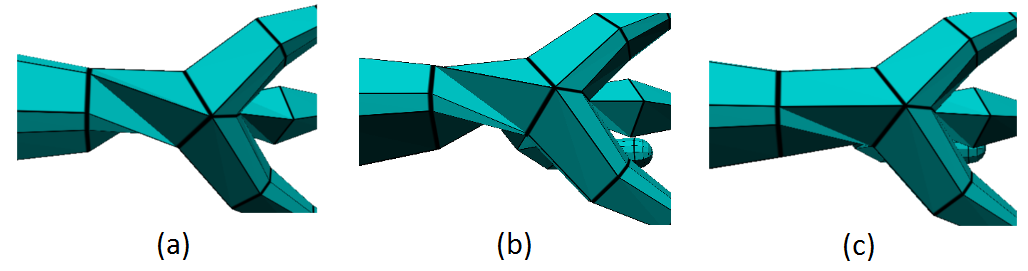
\includegraphics[width=\textwidth]{images/join_pairing.png}
    \caption[BNP joining pairing]{BNP joining pairing. (a) minimal Euclidean distance; (b) minimal angle; (c) minimal total Euclidean distance.}
    \label{fig:join_pairing_ilu}
\end{figure}

\paragraph{Leaf node termination}
As in original paper \cite{sqm} we have decided to terminate leaf nodes with triangular faces. Each face has two vertices from the current one-ring and one vertex is the position of the leaf node.

\section{Final vertex placement}\label{sec:fvp}
We use quaternions calculated during skeleton straightening.
For each skeletal node we accumulate the final rotation in a matrix.
Matrices are used because they are more suitable for GPU calculations than quaternions.
Linear blend skinning, as described in \cite{Kavan-07-SDQ}, is used to combine skinning matrices corresponding to each vertex on GPU.
We apply skinning transformation on GPU in vertex or tessellation shaders.
We have also implemented linear blend skinning on CPU.
This is advantageous for comparison purposes as well as when we are generating base meshes from cyclic skeletons.
Since we are using triangulations on CPU to close generate cyclic skeletons, we need to apply linear blend skinning before the triangulations.
Skinning could be still calculated on GPU and the resulting geometry could be send back to CPU for processing. However, we have found that our generated base meshes are relatively simple and the overhead from transmitting data between CPU and GPU would be more time consuming than CPU implementation of linear blend skinning.

\section{Ellipsoid Nodes}
An ellipsoid can be defined as a sphere with associated transformation matrix.
We take advantage of this representation of ellipsoids.
Instead of more complex ray-ellipsoid intersection that would have to be computed at each ellipsoid node, we have decided to represent each ellipsoid node as a sphere and a transformation matrix.
First our base mesh algorithm is evaluated as described previously with spherical nodes.
After that we send the transformation matrices corresponding to each ellipsoid node to GPU.
The vertices corresponding to each ellipsoid node are transformed directly in vertex shader.
Thanks to this, ellipsoid nodes require minimal extra computing resources from CPU.
The results can be seen in Figure \ref{fig:ellipsoid_ilu}.

\begin{figure}[ht]
    \centering
    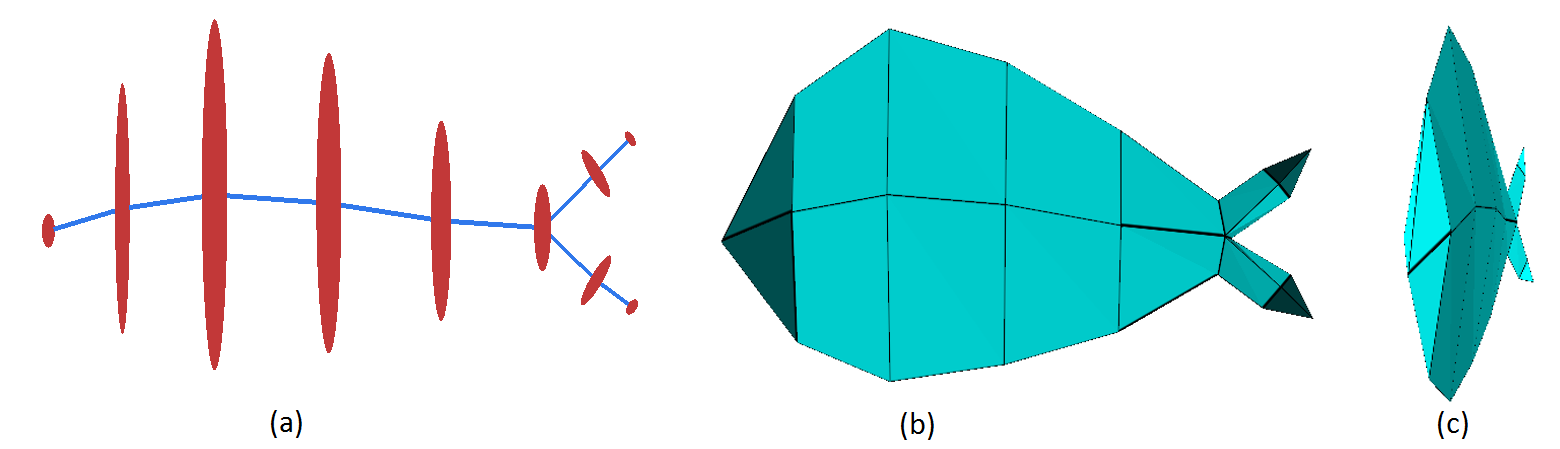
\includegraphics[width=\linewidth]{images/ellipsoid_fish_ilu}
    \caption[Ellipsoid nodes]{Ellipsoid nodes. (a) skeleton with ellipsoid nodes specified; (b) base mesh generated from skeleton; (c) base mesh from different angle.}
    \label{fig:ellipsoid_ilu}
\end{figure}

\section{Tessellation}
Tessellation shaders available since OpenGL 4.0 are used to tessellate the generated base mesh.
Two connected spherical nodes, a parent and a child, implicitly define a truncated cone between them.
The base of the cone has the radius of parent spherical node and the top of the truncated cone has the radius of child spherical node.
Each vertex generated during tessellation is projected onto this cone.
The projection is done by translating the vertex along its normal until it reaches the surfaces of the cone.
Tessellation is shown in Figure \ref{fig:tessellation_ilu}, the generated base mesh is shown in Figure \ref{fig:tessellation_ilu}a and the tessellated base mesh in Figure \ref{fig:tessellation_ilu}b.
However, during this step the generated base mesh gains volume and the newly generated vertices can intersect the tessellated base mesh.
This effect can be seen in Figure \ref{fig:tessellation_ilu}c.
To recover from this situation, we detect sharp vertices in the input mesh and apply a radius scaling scheme.
Sharp vertices are vertices which faces are forming acute angles.
In tessellation shader we have access only to one patch and its vertices.
So we compute the sharpness of each vertex by comparing and thresholding the normal of each vertex with the normal of the patch.
The smaller the angle between vertex normal and patch direction is, the sharper the vertex is.
We apply Bezier curves to modify the radius of the truncated cone.
We use Bezier curves that yield values between $[0;1]$.
For each tessellated vertex its distance from the beginning of the patch is calculated.
The distance is equal to tessellation parameter $v$ computed by the GPU.
Scaling reduction factor is calculated by sampling a point on Bezier curve at point $t = distance$.
The radius of each vertex is then multiplied with calculated factor.
The smoothed mesh is shown in Figure \ref{fig:tessellation_ilu}d.
Currently, the scaling Bezier curve is constant but it could be dynamically changed based on the sharpness of the vertices.

\begin{figure}[ht]
    \centering
    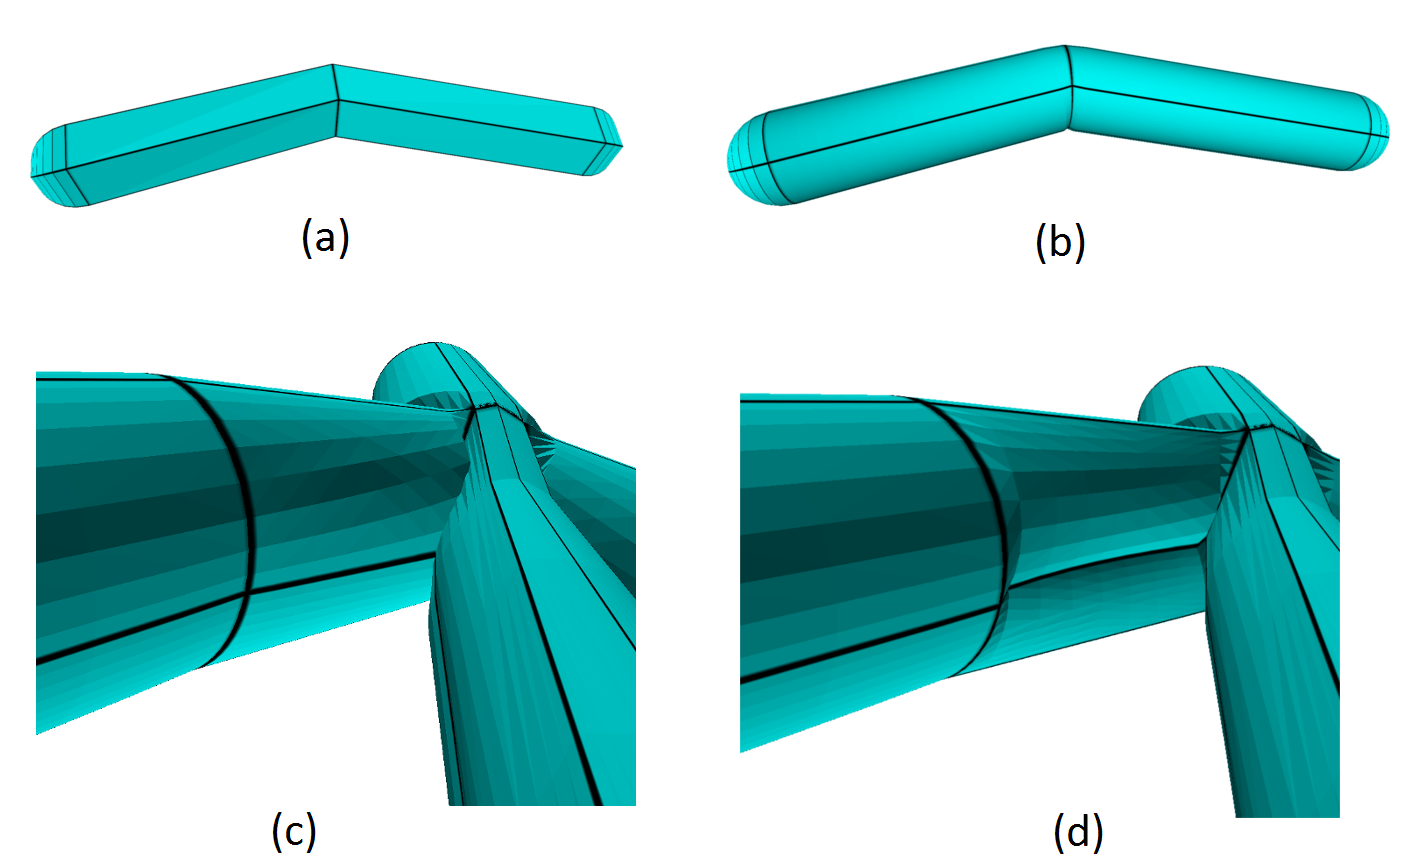
\includegraphics[width=0.9\linewidth]{images/tess_ilu}
    \caption[Tessellation and smoothing]{Tessellation. (a) non-tessellated mesh; (b) tessellated mesh wit 20 subdivisions; (c) tessellated mesh with self intersection; (d) tessellated mesh with radius scaling reduction.}
    \label{fig:tessellation_ilu}
\end{figure}

\section{Capsule Ending}
A capsule is a hemisphere generated at each leaf node of the input skeleton.
This hemisphere replaces the triangle fan pyramid generated by original SQM algorithm.
Generating of capsules can be approached in two ways.
The first is to generate a capsule at each leaf node corresponding to its radius.
The second is inserting additional nodes into the input skeleton with decreasing radius that would approximate a capsule.
We have implemented the second approach because it fits nicely into our pipeline.
Capsules generated this way can be directly tessellated on the GPU without any additional processing.
At each capsule leaf node, we insert additional nodes into the input skeleton proportional to the radius of the capsule node.
The radius of each node is decreased according to Equation \ref{eq:radius_change} where $nodeRadius$ is the radius of capsule node and $step$ is a number between $(0-1]$, that represents the distance from center of the capsule to its edge.
Final tessellated capsule is shown in Figure \ref{fig:capsule_ilu}.

\begin{equation}
newRadius = \sqrt{nodeRadius^{2} * (1 - step^{2})}
\label{eq:radius_change}
\end{equation}

\begin{figure}[ht]
    \centering
    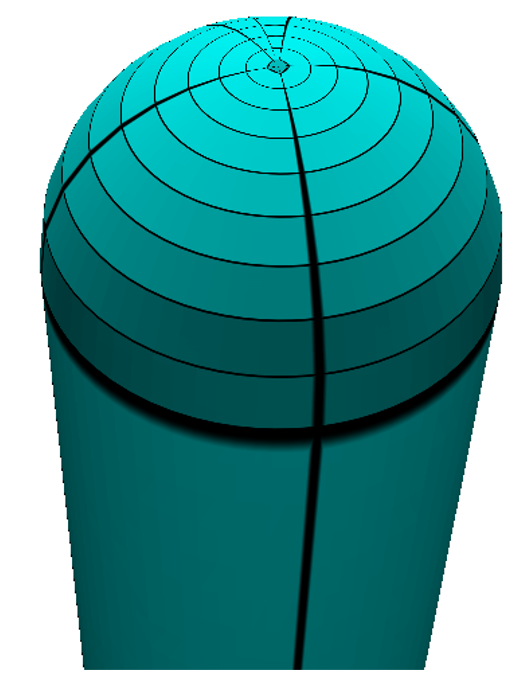
\includegraphics[width=0.5\textwidth]{images/capsule}
    \caption[Capsule generation]{Capsule generated by our algorithm and tessellated on GPU in tessellation shaders.}
    \label{fig:capsule_ilu}
\end{figure}

\section{Linear Skeletons}
Linear skeletons without branch nodes lack the initial geometry that is generated during BNP generation step described in Section~\ref{sec:bnp_gen}.
Additional nodes could be inserted into the input skeleton to form at least one branch node but we have found that it needlessly disturbs the flow of the output mesh.
Instead we decided to use a different approach.
We introduce an additional input parameter $N$ which specifies how many vertices should be generated for each node of the linear skeleton.
This parameter does not decrease the robustness of our approach, because additional vertices are generated during tessellation and the original number of vertices is negligible.

First step of the algorithm is setting the root to be the head of the input linear skeleton.
Next step of the algorithm is straightening of the input linear skeleton.
The input skeleton is shown in Figure \ref{fig:worm_ilu}a.
Next, $N$ vertices are generated around first connection node which is a child of the root node.
These vertices are distributed regularly around the node by slerping a quaternion which center of rotation is nodes position, axis of rotation is the direction from connection node to root node and magnitude is $360/N$.
Newly generated vertices are then joined with other vertices as in original base mesh algorithm.
Leaf nodes form a triangle fan and connection nodes form a tube of quadrilaterals.
The joined linear base mesh is shown in Figure \ref{fig:worm_ilu}b.
Skinning matrices are used to transform the generated linear skeleton into its input pose Figure \ref{fig:worm_ilu}c.

\begin{figure}[ht]
    \centering
    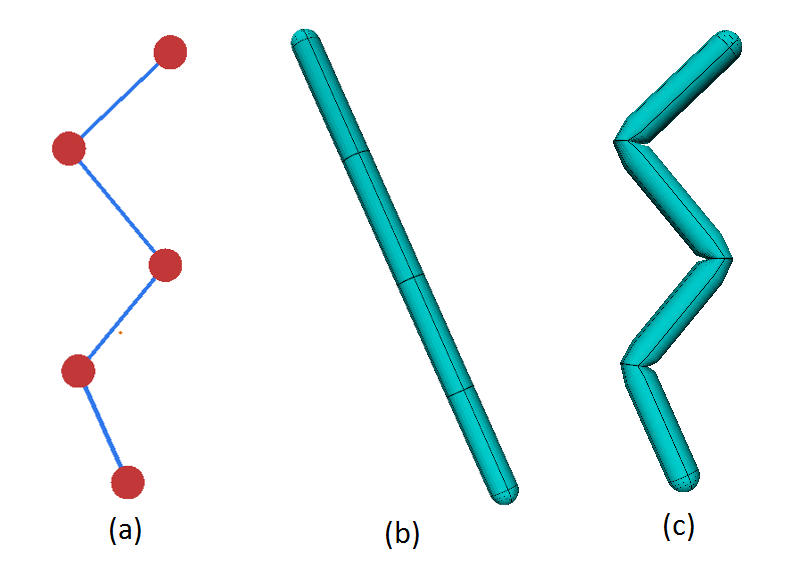
\includegraphics[width=0.7\textwidth]{images/worm_generation}
    \caption[Linear base mesh]{Linear base mesh generation. (a) input linear skeleton; (b) straightened and joined linear skeleton; (c) final linear base mesh.}
    \label{fig:worm_ilu}
\end{figure}

\section{Root That Is Not a Branch Node}
If the root of the input skeleton is not a branch node and a branch node is present in the skeleton, we can find it with a depth first search.
When we have at least one branch node we can re-root the tree so that the located branch node would be the root of the tree.
We apply Algorithm \ref{alg:reroot} to re-root the skeleton.
We want to make the input node the root of the skeleton.
For that it has to have no parent node and all other nodes in the skeleton should have a parent node.
We set the new root to have no parent and store its former parent as $current$ node and the parent of $current$ node as $currentParent$ node.
In a loop we set $currentParent$ as a child of $current$ node.
In order to advance along the skeleton, we set $current$ node to the parent of $current$ node and $currentParent$ node to the parent of $currentParent$ node.
This way we ascend along the skeleton, until we reach the former root node and the algorithm terminates.
\begin{algorithm}[h]
\caption{ReRoot}
\label{alg:reroot}
\begin{algorithmic}
	\STATE{\textbf{Input:} $node$}\COMMENT{the node that should be the new root}
	\STATE{$current \leftarrow node.parent$}
	\STATE{$currentParent \leftarrow current.parent$}
	\STATE{$node.parent \leftarrow NULL$}
	\STATE{$current.parent \leftarrow node$}
	\STATE{$current.removeChild(node)$}
	\STATE{$node.addChild(current)$}

	\WHILE{$current \neq root$}
		\STATE{$current.addChild(currentParent)$}
		\STATE{$parent.removeChild(current)$}
		\STATE{$newParent \leftarrow currentParent.parent$}
		\STATE{$currentParent.parent \leftarrow current$}
		\STATE{$current \leftarrow currentParent$}
		\STATE{$currentParent \leftarrow newParent$}
	\ENDWHILE
	\STATE{$root = node$}
\end{algorithmic}
\end{algorithm}

\section{Cyclic Skeletons}
Our last improvement is generation of base meshes from cyclic skeletons.
The cycle can be placed anywhere in the input skeleton.
The base algorithm could not be modified to allow generation of cyclic meshes because during BNP refinement step of the algorithm a cycle could cause an infinite loop.
However, we can modify the input skeleton in a way that would allow us to generate cyclic skeletons.
As the input we have a cyclic skeleton Figure \ref{fig:cycle_skeleton}.
Cyclic edge is marked with yellow color and cyclic nodes with green and violet colors.

First, we split the cycle by removing the yellow cyclic edge.
To each cyclic node we add an extra child node as shown in Figure \ref{fig:cycle_break}.
Light green node for green cyclic node and pink node for violet cyclic node.
These new nodes serve to preserve the skinning matrices that will rotate tubes generated from cyclic nodes to face each other. This can be seen in Figure \ref{fig:cycle_before}. Base mesh was generated as described in Chapter \ref{ch:proposed_solution} with one exception.
The triangles that should been generated for light green and pink nodes were omitted.
Now the gap between cyclic nodes can be closed.
We first project vertices associated to each cyclic node to a plane with origin at $O(0, 0, 0)$ and normal $n(0, 1, 0)$.
Next, we normalize the vertices so that vertices associated with violet node lie at a circumference with radius 1 and vertices associated with green node lie at circumference with radius 2.
The position of projected points is shown in Figure \ref{fig:cycle_del_before} where vertices associated with green node have green color and vertices associated with violet node have violet color.
Now we execute a Delaunay triangulation on the transformed points.
After the triangulation is done, we exclude triangles generated solely between green or violet vertices.
The remaining triangles represent the faces that should be generated in order to close the gap between cyclic nodes as can be seen in Figure \ref{fig:cycle_del_after}.
Final cyclic mesh is shown in Figure \ref{fig:cycle_after}.

%\begin{figure}[ht]
%    \centering
%    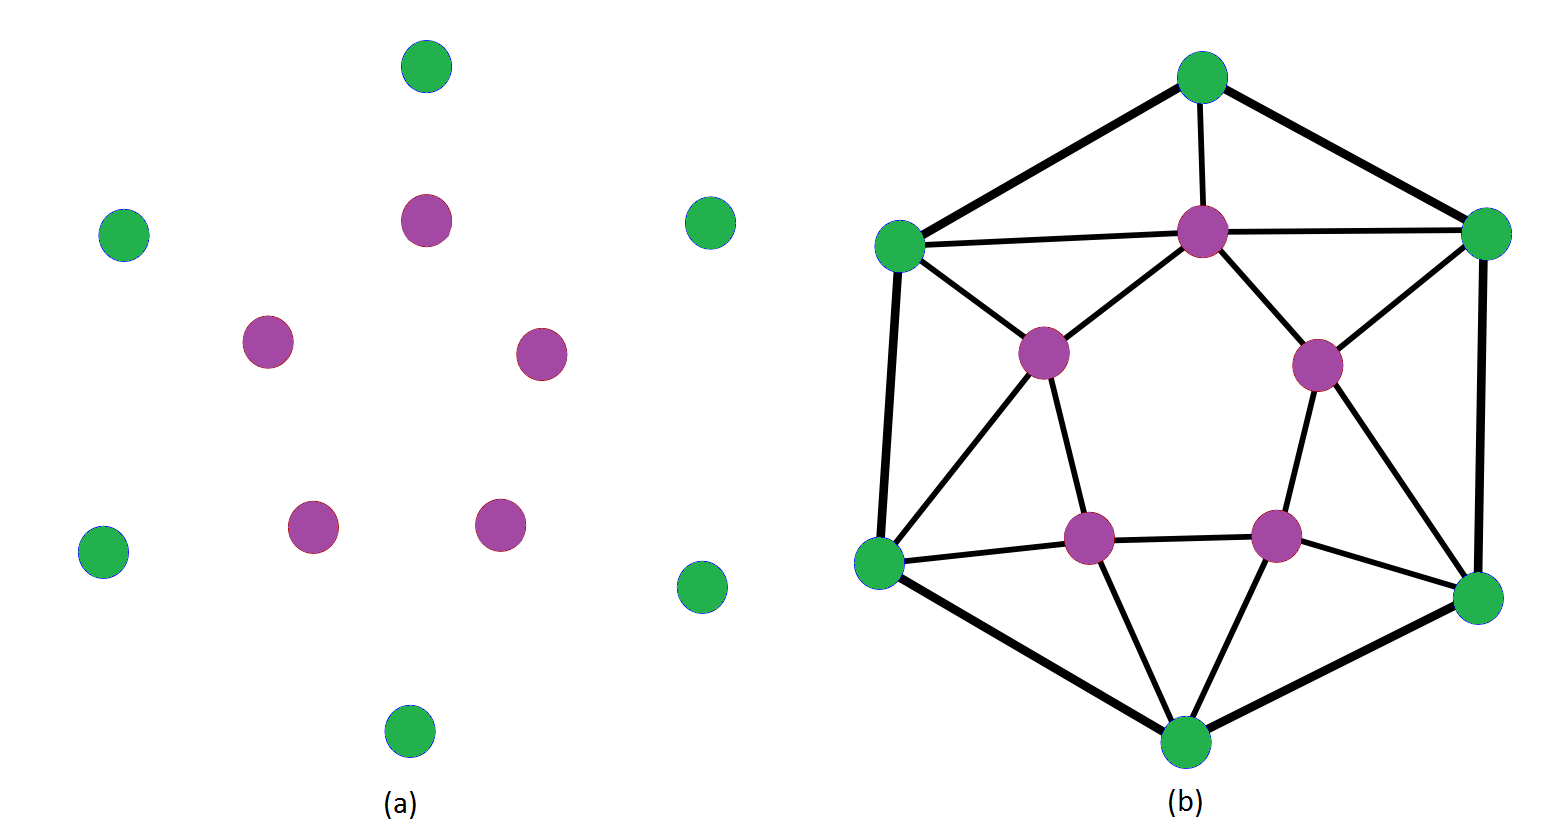
\includegraphics[width=0.7\textwidth]{images/cycle_del}
%    \caption[Delaunnay triangulation closing cyclic mesh]{Delaunnay triangulation of input points (a) used to generate faces between vertices forming the cycle (b); Green points represent vertices corresponding to cycle node 1 and violet represent vertices of cycle node 2 from Figure \ref{fig:cycle_ilu}.}
%    \label{fig:del_ilu}
%\end{figure}
%
%\begin{figure}[ht]
%    \centering
%    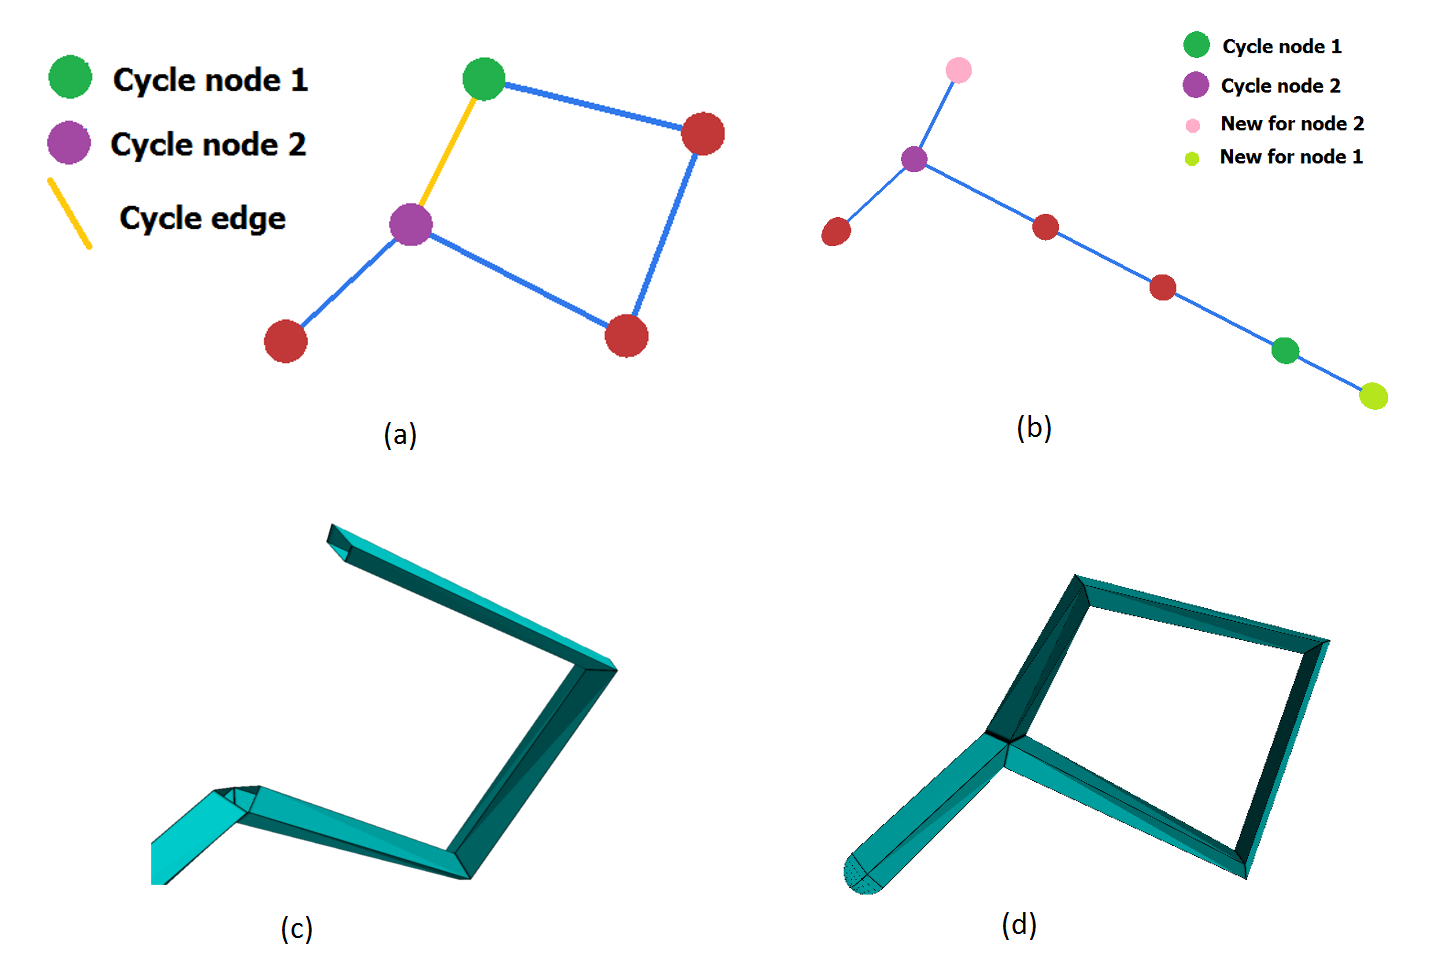
\includegraphics[width=\textwidth]{images/cyclic_skeletons}
%    \caption[Cyclic skeleton generation overview]{Cyclic skeleton base mesh generation. Cyclic skeleton, cyclic edge marked with yellow color, cyclic nodes with green and violet (a); Split cycle with one inserted node for each former cyclic nodes lightgreen for green node and pink for violet node (b); Generated base mesh before the cycle is closed (c); Generated base mesh after the cycle is closed (d).}
%    \label{fig:cycle_ilu}
%\end{figure}

\begin{figure}[ht]
        \centering
        \begin{subfigure}[b]{0.4\linewidth}
        \centering
			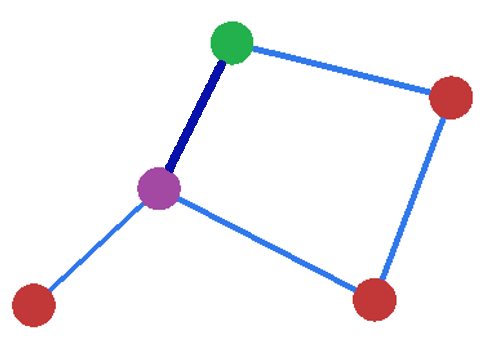
\includegraphics[width=0.9\linewidth]{images/cyclic_skeletons_1}
            \caption{Cyclic skeleton, cyclic edge marked with yellow color, cyclic nodes with green and violet}
            \label{fig:cycle_skeleton}
        \end{subfigure}%
        ~ %add desired spacing between images, e. g. ~, \quad, \qquad etc.
          %(or a blank line to force the subfigure onto a new line)
        \begin{subfigure}[b]{0.4\linewidth}
        \centering
			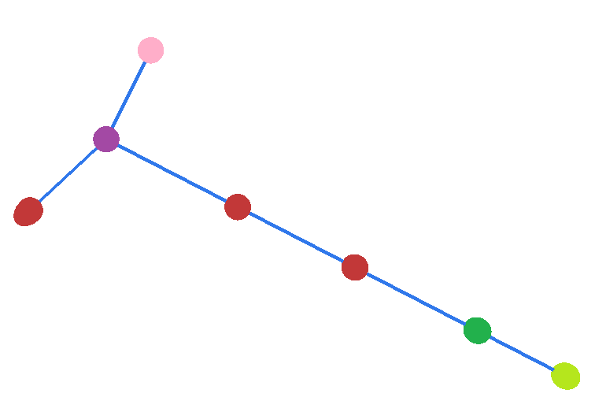
\includegraphics[width=0.9\linewidth]{images/cyclic_skeletons_2}
            \caption{Split cycle with one inserted node for each former cyclic nodes light green for green node and pink for violet node}
            \label{fig:cycle_break}
        \end{subfigure}
        \\ %add desired spacing between images, e. g. ~, \quad, \qquad etc.
          %(or a blank line to force the subfigure onto a new line)
        \begin{subfigure}[b]{0.4\linewidth}
        \centering
			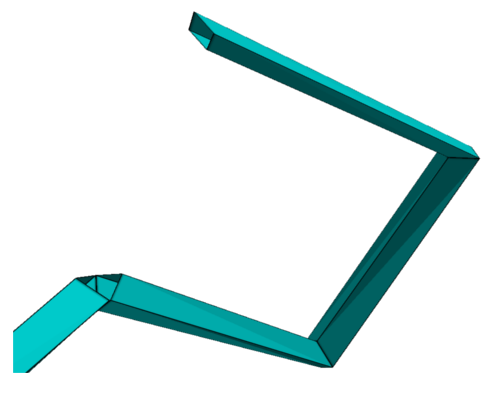
\includegraphics[width=0.9\linewidth]{images/cyclic_skeletons_3}
            \caption{Generated base mesh before the cycle is closed}
            \label{fig:cycle_before}
        \end{subfigure}
        ~ %add desired spacing between images, e. g. ~, \quad, \qquad etc.
          %(or a blank line to force the subfigure onto a new line)
        \begin{subfigure}[b]{0.4\linewidth}
        \centering
			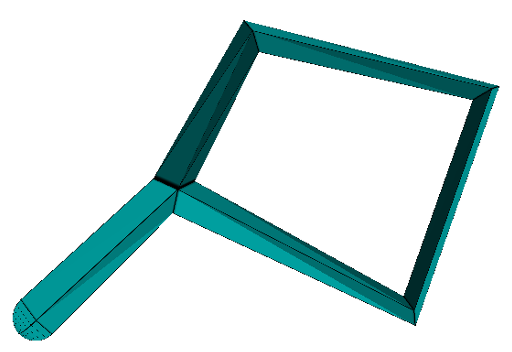
\includegraphics[width=0.9\linewidth]{images/cyclic_skeletons_4}
            \caption{Generated base mesh after the cycle is closed}
            \label{fig:cycle_after}
        \end{subfigure}
        \\ %add desired spacing between images, e. g. ~, \quad, \qquad etc.
          %(or a blank line to force the subfigure onto a new line)
        \begin{subfigure}[b]{0.4\linewidth}
        \centering
			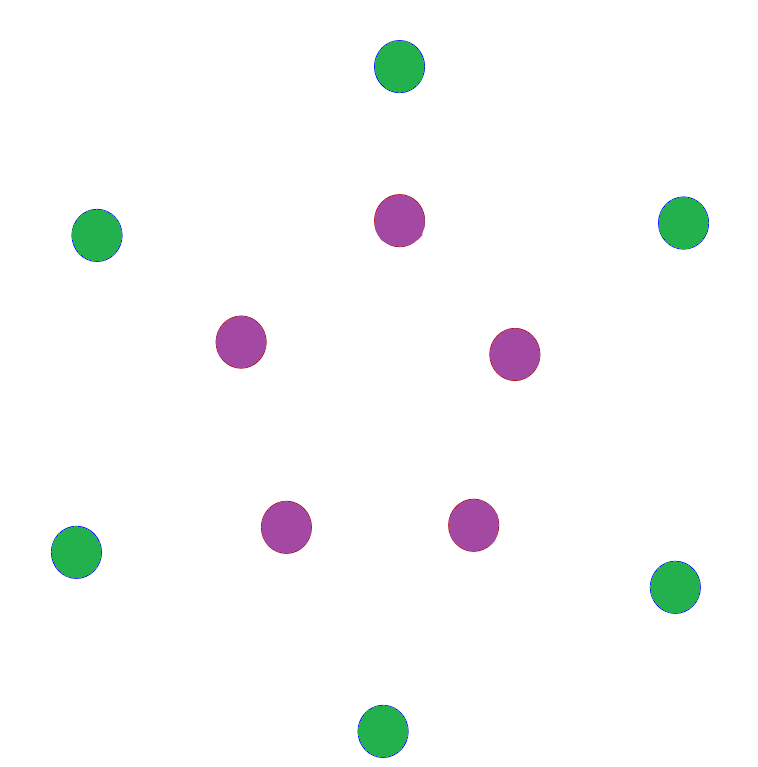
\includegraphics[width=0.8\linewidth]{images/del_tria_1}
            \caption{Vertices corresponding to green and violet cyclic nodes projected onto the same plane}
            \label{fig:cycle_del_before}
        \end{subfigure}
        ~ %add desired spacing between images, e. g. ~, \quad, \qquad etc.
          %(or a blank line to force the subfigure onto a new line)
        \begin{subfigure}[b]{0.4\linewidth}
        \centering
			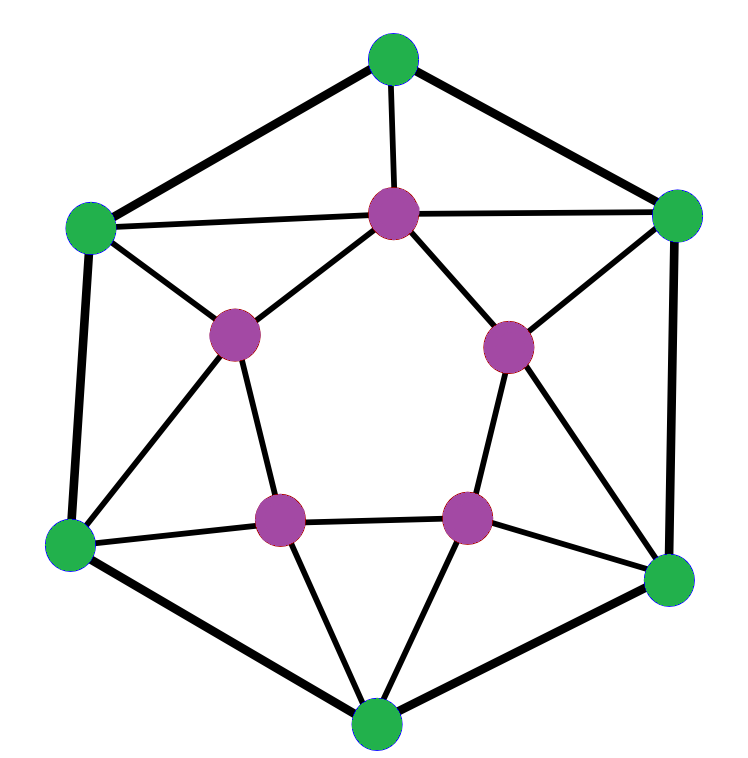
\includegraphics[width=0.8\linewidth]{images/del_tria_2}
            \caption{Faces generated by triangulation that will be used between original unprojected vertices}
            \label{fig:cycle_del_after}
        \end{subfigure}
        \caption{Cyclic skeleton base mesh generation.}
        \label{fig:cycle_ilu}
\end{figure}


\chapter{Implementation}

We have implemented a system, where users can load and edits skeletons from files, or start by scratch from one skeletal node.
Our system is based on model-view-controller pattern.
Model is stored in $BMMAlgorithm$ and $BMMNode$ classes.
These classes take care of storing the skeleton, exporting skeleton to different formats and executing the base manifold mesh algorithm.
Controller is represented by $BMMController$ class.
This class prepares data from model for visualization and handles input from view.
View consists of two parts.
First, is $OpenGL$ window, which displays data provided from controller.
Second, is a Windows form, that provides Graphical User Interface (GUI) elements, which serve to make input easier.

In this chapter we will describe how we implemented our solution.
We will start with used programming language, Integrated Developer Environment (IDE), tools and libraries.
Next, we will describe implemented classes, grouped by model-view-controller pattern in greater detail.
After that we will show some programmable shaders used in our implementation.
Finally, we will describe our implementation of base manifold mesh library.

\section{Programming Language, IDE, Tools, and Libraries}

We have selected C++ as programming language.
The main reasons are that C++ is fast and well established programming language.
Also the open source libraries that we intended to use are available for C++ and many of them are available exclusively for C++.
As IDE we are using Visual Studio 2012, which was the newest version of Visual Studio, when we started our work.
Visual Studio is supported by all of the used libraries.
We have used nVidia nSight for Visual Studio 2012 that is a debugger for graphics cards, which allows to set breakpoints in shaders during execution. We have also used several open source libraries in our project. We will briefly describe the key libraries.
To program the GPU we use OpenGL Shading Language (GLSL) version 4.3.

\begin{itemize}
	\item \textbf{Boost \cite{Boost}} Boost is a set of libraries encapsulating various task like basic input output system, smart pointers, serialization, matrices, etc. We use Boost primary for class serialization. Thanks to boost we can serialize classes into XML files, which can be stored and loaded from disk. This XML files can even be shared between different applications, so we can import skeletons from third party programs.
	\item \textbf{OpenMesh \cite{OpenMesh}} Is an open source half edge data structure library. We use it to store all meshes in our applications. OpenMesh library is capable of storing meshes composed solely from triangles as well as meshes composed of arbitrary polygons. OpenMesh has pre-calculated many convenient iterators for one-ring neighbourhoods, faces and edges adjacent to a vertex, etc. The library is also capable of exporting stored meshes into Wavefront .obj files.
	\item \textbf{GLEW \cite{glew}} The OpenGL Extension Wrangler Library (GLEW) provides efficient run-time mechanisms for activating OpenGL extensions. We use this library to expose OpenGL 4.3 functionality to our application.
	\item \textbf{OpenGL \cite{opengl}} Open source cross platform application programming interface. We use it to leverage the computation capability of GPUs to achieve hardware accelerated rendering.
	\item \textbf{GLM \cite{glm}} OpenGL Mathematics library that provides the same vector and matrix operations as available in GLSL. GLM also provides several function, that are deprecated in newer versions of OpenGL. We use this library to manipulate camera, model matrices, and for general matrix computations. GLM library is also capable of quaternion computations that are used during smoothing of BNPs and during computation of skinning matrices.
\end{itemize}

\pagebreak

\section{Classes}

Each class implements its functionality as interfaces.
These interfaces encapsulates underlying algorithms.
This allows us to replace algorithms, without affecting the rest of the code.
The relationships between the most important classes are shown in Figure \ref{fig:classes}.
Model provides interface for the controller, which allows to query models data, for visualization.
The interface provided by model also allows to change its state and attributes of various classes.
View provides an interface for the controller, which allows the controller to display models data.
Views is also capable of receiving users input, either via mouse or by setting values exactly in an inspector panel.
Controller connects model and view together.
At constant intervals, data from model and input from view are gathered.
The model is updated according to users input and the data changes are immediately reflected in the view.

\begin{figure}[h]
    \centering
    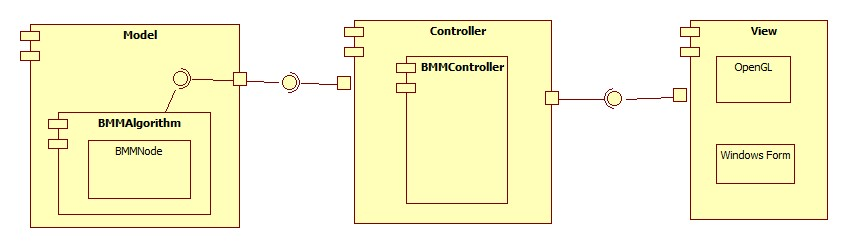
\includegraphics[width=\textwidth]{images/classes}
    \caption[Component diagram of classes]{Component diagram of most important classes, forming the model-view-controller pattern.}
    \label{fig:classes}
\end{figure}

\subsection{Model}

Model stores the data required for our algorithm, that is the input skeleton.
Model can be in six different states, five of which mirror the steps of base mesh algorithm.
The states are: skeleton editing, skeleton straightening, BNP generation, BNP refinement, BNP joining and final vertex placement.
To input a skeleton and display the corresponding generated base mesh only skeleton editing and final vertex placement would be adequate.
However the remaining states are useful for visualization of the algorithm.
The model is designed like a library, that means it is independent from view and controller and base mesh generation can be distributed as a library.

In skeleton editing state, the input skeleton is accessible for editing.
New nodes can be added to skeletal structure.
Existing nodes can be moved, their corresponding sphere can be specified, transformation matrices can be set and leaf nodes can be set to capsules or triangle fans.
Also cyclic edges between two nodes can be specified in this state.
Outside of this state user can not edit the input skeleton by any means.

After entering skeleton straightening state the preprocessing step skeleton straightening is executed and the resulting straightened skeleton is displayed.
User can inspect the effect that skeleton straightening has on the input skeleton.

Upon entering BNP generation state the corresponding algorithm stage is executed.
User can now see polyhedrons, corresponding to each branch node, generated by spherical Delaunnay triangulation.
User can inspect faces of generated polyhedrons and display their normals.

In BNP refinement state user can see refined and smoothed polyhedrons generated by our algorithm.
The refinement procedure can be changed, after which the algorithm will be recomputed and polyhedrons smoothed with different smoothing scheme will be shown to the user.

In BNP joining state the equally named step of our algorithm is executed.
User can see straight base mesh and display normals corresponding to its faces.
It is also possible to tessellate the straightened base mesh.
The tessellation factor is global and can be adjusted from GUI.
Since the last step of the algorithm was not yet executed, elliptical nodes would appear as spherical nodes.

After entering final vertex placement state, the last step of the algorithm is executed.
User can see the final output base mesh and adjust tessellation factor.
Elliptical node have their corresponding transformations applied.
After executing any step of the base mesh algorithm user can return to any previous state, which will re-execute the algorithm again.
Application work flow is depicted in Figure \ref{fig:states}.
Direct transitions between states represent steps of the base mesh algorithm.
Transitions through junction node represent the possibility to jump between any two states in the application.

\begin{figure}[h]
    \centering
    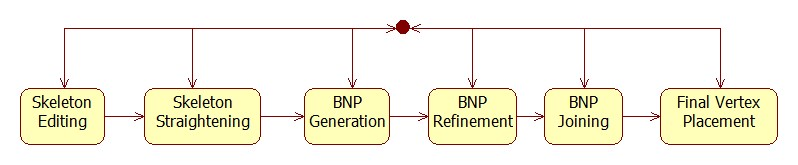
\includegraphics[width=\textwidth]{images/states}
    \caption[Model state diagram]{State diagram of model. Arrows between states show application work flow. Transition between any states is possible through the junction node.}
    \label{fig:states}
\end{figure}

\subsubsection{BMMNode}

BMMNode is main class of the model that holds the input skeleton.
It is represented as an oriented rooted graph.
The root of the graphs is stored in BMMAlgorithm class.
The steps of base mesh algorithm are implemented in BMMNode class as recursive functions.
The functions first process the root node and then continue, with its child nodes.
All necessary data for drawing, tessellation and subsequent algorithm steps are also accessed recursively from skeletons root. All important variables are stored directly in nodes: input skeleton node position, generated polyhedron, skinning weights and other attributes required for the execution of base mesh algorithm.

\subsubsection{BMMAlgorithm}

BMMAlgorithm class provides interface that hides the underlying oriented graph and implements states discussed previously.
All queries to BMMAlgorithm are forwarded to the root node, which recursively produces output, that BMMAlgorithm returns.
This way if we would later decide to change base mesh algorithm in any way basic functionality would still be accessible through BMMALgorithm.
Furthermore BMM algorithm computes certain pre and post processing that simplifies algorithms in BMMNode.
BMMAlgorithm implements the re-rooting algorithm, so we do not need to check for invalid parents in recursive functions.
The rooted oriented graph is stored twice in BMMAlgorithm.
One copy is used to execute the base mesh algorithm itself and the other copy is used to stores the input of the algorithm, so that it can be re-executed.

\subsection{View}

View consist of Windows form components and an OpenGL view.
Windows form components are managed by Visual Studio and we are synchronizing them with our controller.
Models state is displayed in a view with OpenGL 4.3 context.
Mouse interaction in OpenGL view is recorded by our GLInput class.

\subsubsection{OpenGL view}

OpenGL view periodically queries controller for changes in model.
If model changed its state, or input skeleton was modified OpenGL view reloads buffers with new data from the model.
Otherwise view displays previously stored data.
This reduces unnecessary commands to reload buffers with data that is already stored.
Buffers are filled with data and active OpenGL programs are selected depending on models state.

In skeleton input and skeleton straightening states, buffers are filled with lines connecting skeletal nodes and spheres corresponding to each node.
Elliptical nodes transformation matrices are also stored in buffers.
Two shader programs are used to render skeletal structures.
One is specifically designed for line drawing.
The other is designed for sphere drawing.
In order to reduce the amount of data required to be send to GPU during node rendering, only one model of an icosahedron is send to GPU.
This model is then tessellated and smoothed to resemble a sphere.
Corresponding model matrices are used to position the tessellated sphere at skeleton nodes position, with appropriate scale.

BNP generation and BNP refinement states also share the same shader programs.
Upon entering these states all polyhedrons are queried from the model.
The queried polyhedrons are converted from half edge representation to indexed face representation and stored in buffers on GPU.
The shader program, responsible for rendering of polyhedrons, features one-pass wireframe rendering and uniform shading for each triangle.
This settings are useful for visualization of generated polyhedrons.

In the last two states BNP joining and final vertex placement, the generated base mesh is converted from half edge to indexed face.
Quadrilateral parts of the mesh are send as quadrilaterals to GPU for tessellation.
Shader program for base mesh rendering displays uniformly shaded faces and wireframe.
The shader program is also capable of Linear Blend Skinning computations, that transform the input mesh.
Currently they are used only to revert transformations applied during skeleton straightening.

\subsubsection{GLInput}

When users clicks in OpenGL view the position in view and mouse button are registered.
Mouse position is then converted from 2D view coordinates to 3D camera coordinates.
A ray with origin at mouse 3D projection and direction from camera to mouse 3D projection is casted in the scene.
The process is shown in Figure \ref{fig:camera_selection}.
The mouse 2D location was mapped onto near plane and yellow ray was casted into the scene.
The first hit object is then selected.
Mouse actions are context dependant.

If the ray intersects a node the node is selected, its corresponding attributes are displayed in the inspector.
A selected node can be moved in the scene and this way its position attributes are updated.
With selected node user can create new nodes as child of selected node with middle click of the mouse.
Right clicking on a different node creates a cycle between selected and clicked node.
User can also rotated child nodes of a node.
In this mode left, right and middle clicks produce rotations around X, Y and Z axis respectively.

If after tracing the ray we do not encounter a node the resulting interaction is handled as rotations and translations of camera.
Camera is locked on a point and can be rotated around that point by right clicking in the scene.
A left click moves the point in a plane that is parallel to near plane of the camera.
Mouse wheel translates the camera along its view direction and therefore produces the effect of zooming in and out with the camera.

\begin{figure}[h]
    \centering
    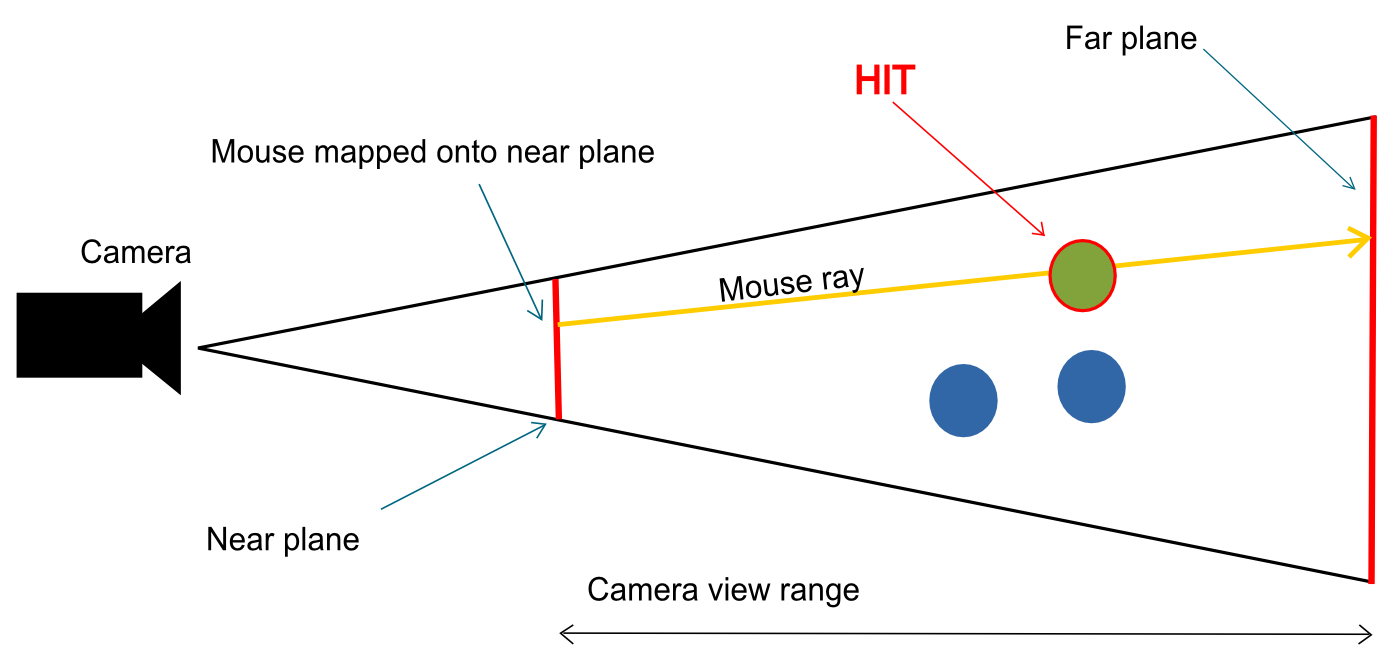
\includegraphics[width=\textwidth]{images/camera_selection}
    \caption[Camera selection]{Camera selection in 3D. Mouse 2D location is mapped onto near plane and a ray is casted through the scene. The first object hit by the ray is selected.}
    \label{fig:camera_selection}
\end{figure}

\subsection{Controller}

Controller is represneted by BMMController class.
BMMController connects model and view together by updating input forms with models data, providing OpenGL view with buffer data from the model and if new values are provided through input forms or mouse interaction, controller updates model accordingly.
Controller also handles file input and output.
When an input skeleton is loaded from a file, controller de-serializes objects saved in file and creates new BMMNode.
This new node is then set as the root for BMMAlgorithm.
BMMController is also capable of saving current skeleton into a file.
First controller queries BMMAlgorithm for skeletal representation through a provided interface.
Then controller serializes and stores the received skeletal structure.
Through a different interface, BMMController can query the generated base mesh, represented as Wavefront .obj and store it in a file.
Since controllers only interaction with model is providing input and output, it can be replaced at any time to accommodate for a different application.
For example in a library for base manifold mesh generation, where a one-shot algorithm would be desired, the controller would  send input skeleton to BMMAlgorithm.
Let BMMAlgorithm execute and return the generated base mesh either as a Wavefron .obj suitable for storing or transferring to a different application, indexed face data structure suitable for rendering or in half edge data structure suitable for further mesh processing.

\section{GPU Shaders}

GPU shaders are used to program graphics hardware.
With shaders one can control the position of rendered vertices, lighting in scene and even compute certain calculation directly on GPU.
Since we are using OpenGL API to draw geometry, we are also using OpenGL Shading Language (GLSL) to program graphics hardware.
We are programming in GLSL version 430, which was released along with OpenGL 4.3.
We choose this version of GLSL because of two main reasons.
First, is that we wanted to use tessellation shaders that are available only in GLSL 400 and newer.
The second reason is that GLSL 430 offers various advantages to previous 4XX versions.
The main advantages comes from more extensive usage of layout qualifiers, which simplify application code.
New layout qualifiers allow us to bind texture units, shader uniforms and per-vertex attributes directly in shaders.
Application responsibility then becomes to send data to graphics card in appropriate order.
Shaders can be linked together to form a program that is responsible for drawing on GPU.
Each type of shader can be presented in a program only once.
GLSL version 430 features these types of shaders, listed in order of execution:
\pagebreak
\begin{itemize}
	\itemsep-0.25em 
	\item \textbf{Vertex Shader} - must be implemented in every shader program. Its purpose is to transform position of vertices sent to GPU.
	\item \textbf{Tessellation Control shader} - optional shader. Sets the level of tessellation that should be produced by hardware.
	\item \textbf{Tessellation Evaluation shader} - optional shader. Its main purpose is to adjust the position of vertices generated by tessellation.
	\item \textbf{Geometry shader} - optional shader. Serves to generate new geometry directly on graphics hardware.
	\item \textbf{Fragment shader} - must be implemented in every shader program. Defines the color of each fragment, from its material, lighting, etc.
\end{itemize}
We have implemented various specialized shaders.
In this section we will describe the most interesting and important of our implemented shaders.

\subsection{Skinning and Ellipsoid Nodes}

Linear Blend Skinning is a technique of animating characters.
As we described previously, we can compute final vertex placement as an animation, from straightened skeletons pose to input skeletons pose.
There are two attributes needed for Linear Blend Skinning: skinning matrices derived from rotation of bones around their degrees of freedom and per-vertex weights.
The weight resemble how much is a vertex influenced by each matrix.

For our case a vertex can not be influenced by more than two skinning matrices.
The first is rotation of a bone from bind pose (straightened skeleton) to reference pose (input skeleton).
The second matrix is matrix representing the rotation of the next bone from bind to reference pose.
This combination of matrices produces junctions that are not self collapsing.
Since we are using only two matrices per vertex, most of the matrices have assigned a weight of 0, so we can send as per-vertex data only weight for actually used matrices.
We are only sending weights for used matrices we also need to send index for each used matrix.
In practice GLSL reserves for each per-vertex attribute a space that can hold a vector of four components.
So we are sending four weights and four indices for each vertex, even though only two of them are used, this can potentially allows us to use more complex skinning animations if we so desire.
Skinning matrices can be send to GPU in two ways.
The former is to send skinning matrices as uniforms, the latter is sending them in a texture.
Sending skinning matrices via textures is more general approach as a shader could be compiled just once and used for models with arbitrary number of bones.
However accessing uniforms in shaders is much faster that accessing textures and a shader needs to be compiled just once for each object.
Alternatively if we are sending matrices in shader uniforms we can reserve space needed for the object that requires most matrices and compile shaders only once.
For our implementation we only need do display one object, so we decided to send skinning matrices to GPU via shader uniforms, due to the efficiency of the method compared to textures.

We have implemented Linear Blend Skinning in vertex and tessellation evaluation shaders.
Vertex implementation resembles most a CPU implementation, as for the rest of the graphics pipeline vertex positions are equal.
We also implemented Linear Blend Skinning in tessellation evaluation shaders in order to compare visual results of skinning vertices after they have been tessellated.

\subsubsection{Vertex Shader Implementation}

The source code is shown in Listing \ref{lst:vert_skin}.
For each vertex we combine all matrices influencing said vertex into one.
We transform vertex and its normal with compound transformation matrix.
This way the vertex is transformed equivalently to a CPU implementation.
Since we also want to generate ellipsoid nodes, we send a transformation matrix for each node.
Because the number of nodes is the same as the number of skinning matrices, we can safely use an array of the same length for both skinning and transformation matrices.
Transformations are specific for each node, which means that transformation matrices do not need to be combined nor weighted.
To optimize the number of data send to GPU we store ids of skinning matrices in a specific order.
The first id is always the id of a transformation matrix that should be applied on currently precessed vertex.

\linespread{1.2}
\begin{lstlisting}[language=GLSL,caption={Linear Blend Skinning implemented in vertex shader},label={lst:vert_skin}]
/*                        Vertex Shader                      */ 
#version 430
//number of matrices filled in before compilation
#define SKINNING_MATRICES fill_in_skinnig_matrices_number
//input variables
layout (location = 0) in vec3 Position;
layout (location = 1) in vec3 Normal;
layout (location = 2) in ivec4 id;
layout (location = 3) in vec4 w;
//shader uniform variables
uniform mat4 MVPMatrix;
uniform mat4 SkinningMatrices[SKINNING_MATRICES];
uniform mat4 TransformMatrices[SKINNING_MATRICES];
//shader main function
void main(void) {
	vec4 pos = vec4(Position, 1.0);
	vec4 normal = vec4(Normal, 0.0);
	//skinning
	mat4 M = (w.x*SkinningMatrices[id.x]
		+ w.y*SkinningMatrices[id.y] 
		+ w.z*SkinningMatrices[id.z] 
		+ w.w*SkinningMatrices[id.w]);
	pos = M * pos;
	normal = M * normal;
	//ellipsoid transformations
	pos = TransformMatrices[id.x] * pos;
	normal = normalize(TransformMatrices[id.x] * normal);
	//output position
	gl_Position = MVPMatrix * pos;
}
\end{lstlisting} 
\linespread{1.5}

\subsubsection{Tessellation Evaluation Shader Implementation}

In tessellation evaluation shader new vertices and faces are generated.
For each tessellated patch we have access to the former vertices that existed before tessellation took place.
Each of this vertices has its corresponding matrices and weights assigned.
However the new vertices do not.
We used two approaches to propagate skinning information from original patch vertices to newly generated vertices.

According to patch vertex order shown in Figure \ref{fig:tess_patch}, we can apply skinning information corresponding to the second patch vertex to all newly generated vertices.
This way the new vertices would be oriented directly towards the last vertices of each patch.
Source code of this approach is shown in Listing \ref{lst:te_last_skin}.
First a matrix is determined depending on parameter $v$.
Vertices lying on patch borders have applied the same skinning transformations as patch vertices.
The new vertices do not use the second transformation matrix, because they are not directly joined to a different bone and do not need to be equally split between two bones.

\linespread{1.2}
\begin{lstlisting}[language=GLSL,caption={Linear Blend Skinning implemented in tessellation evaluation shader, using only skinning information from the first patch vertex.},label={lst:te_last_skin}]
vec3 skinningLastOnly(in vec4 pos, in float v, in ivec2 id0, in ivec2 id1, in vec2 w0, in vec2 w1, in mat4 SkinningMatrices[SKINNING_MATRICES]) {
	mat4 M;
	if (floatEqual(v, 0)) {
		//vertices from patch begining
		M = (w0.x*SkinningMatrices[id0.x] +
			 w0.y*SkinningMatrices[id0.y]);
	} else if (floatEqual(v, 1)) {
		//vertices from patch end
		M = (w1.x*SkinningMatrices[id1.x] +
			 w1.y*SkinningMatrices[id1.y]);
	} else {
		M = SkinningMatrices[ids1.x];
	}
	return M * pos;
}
\end{lstlisting} 
\linespread{1.5}

Second approach is averaging of all skinning data corresponding to patch vertices.
This effect produces smoother transitions between bones.
However smoother transitions limit the curvature of each bone, so they can deviate from the input skeleton, when compared to previously described skinning methods.
The source code is shown in Listing \ref{lst:te_avg_skin}.
The input vertex is transformed by each matrix and the combined to one vertex using skinning weights and its $v$ coordinate.

\linespread{1.2}
\begin{lstlisting}[language=GLSL,caption={Linear Blend Skinning implemented in tessellation evaluation shader, with avaraging of skinning information from all patch vertices.},label={lst:te_avg_skin}]
vec3 skinningAvarage(in vec4 pos, in float v, in ivec2 id0, in ivec2 id1, in vec2 w0, in vec2 w1, in mat4 SkinningMatrices[SKINNING_MATRICES]) {
	vec4 pos0, pos1;
	//lower patch skinning matrices
	pos0 = SkinningMatrices[id0.x] * pos;
	pos1 = SkinningMatrices[id0.y] * pos;
	vec4 t1 = w0.x*pos0 + w0.y*pos1;
	//upper patch skinning matrices
	pos0 = SkinningMatrices[id1.x] * pos;
	pos1 = SkinningMatrices[id1.y] * pos;
	vec4 t2 = w1.x*pos0 + w1.y*pos1;

	return (1-v)*t1 + v*t2;
}
\end{lstlisting} 
\linespread{1.5}

The resulting tessellated meshes are shown in Figure \ref{fig:tess_skin_comp}.
Mesh skinned in vertex shader Figure \ref{fig:tess_skin_comp}a produces visual artifacts at each node of the skeleton.
Last only tessellation evaluation skinning Figure \ref{fig:tess_skin_comp}b reduces visual artifacts and keeps the volume of the input.
Avarage tessellation evaluation shader skinning Figure \ref{fig:tess_skin_comp}c produces the smallest number of visual artifacts.

\begin{figure}[h]
    \centering
    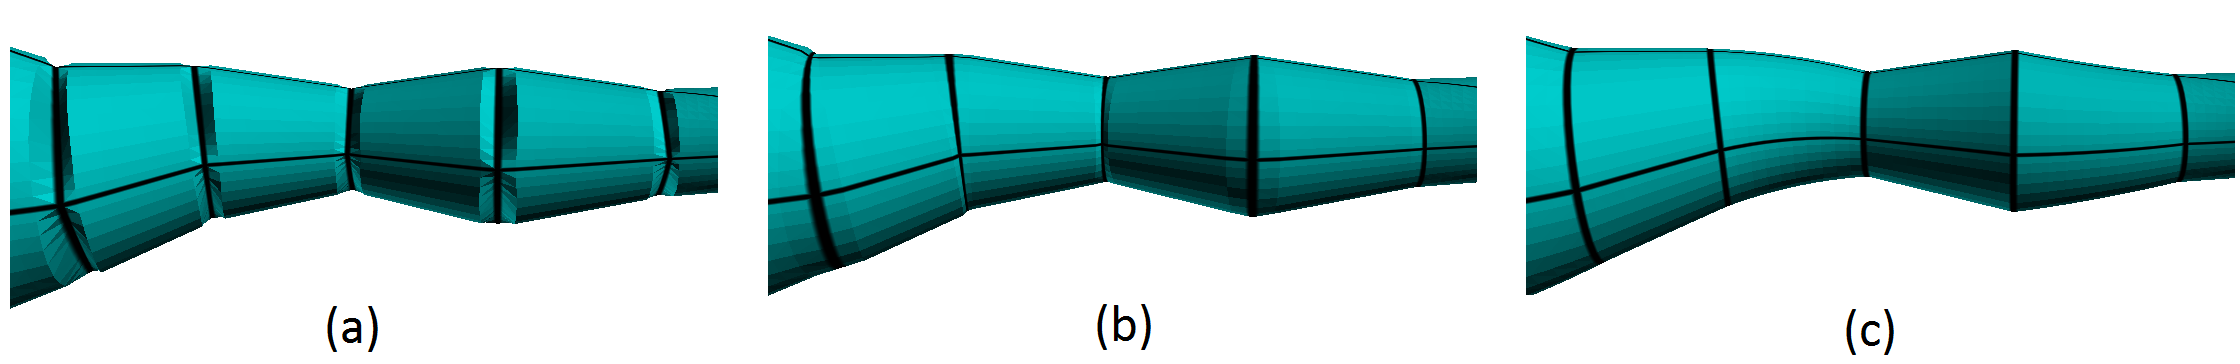
\includegraphics[width=\textwidth]{images/tess_comp}
    \caption[Skinning and Tessellation]{Effects of selected skinning method on tessellation results. (a) vertex shader skinning; (b) last only tessellation evaluation shader skinning; (c) all average tessellation evaluation shader.}
    \label{fig:tess_skin_comp}
\end{figure}

\subsection{Tessellation and Smoothing}

If tessellation is enabled OpenGL is rendering patches instead of triangles.
A patch can be composed of arbitrary number of vertices, however the number must be constant among all rendered patches.
Since we are tessellating quadrilaterals our patch is composed from four vertices.
Our patch is depicted in Figure \ref{fig:tess_patch}.
Vertices forming the patch are in counter-clockwise order starting with v0.
Uv coordinates are displayed with blue and red, respectively.
These coordinates are used to determine the position of new vertices generated during tessellation.

\begin{figure}[h]
    \centering
    \includegraphics[height=15em]{images/tess_patch}
    \caption[Tessellation patch]{A patch used to draw during tessellation. Patch vertices are marked with black, uv coordinates on patch are shown in blue and red respectively.}
    \label{fig:tess_patch}
\end{figure}

The new vertices lie on the same plane as the original quadrilateral.
Because of that in order to have any meaningful results, we also need to process the generated vertices.
We could use an already existing GPU subdivision algorithm for example subdivision approximation with Gregory patches \cite{gregory_patch}, or adaptive tessellation of subdivision surfaces presented in \cite{gpu_gems_2}.
However both of these algorithms are fairly complex, so we decided to use a simpler approach.

Each node has a defined sphere, so that between each pair of nodes lies a truncated cone.
We can sample the radius of truncated cone along its height, which corresponds to v coordinate and simply project each new vertex onto the truncated cone.
This way newly inserted vertices would have corresponding radius according to the input skeleton.
An example of such a shader is shown in Listing \ref{lst:tess_proj}.
However with this procedure the tessellated mesh gains volume, which could lead into self intersection.
In order to avoid this self intersection we are smoothing patches whose vertices have too sharp angles and therefore could potentially intersect with another patch.
We are using ease-in, ease-out and ease-in-out, depending on if the bottom patch vertices (v0, v3), upper patch vertices (v1, v2) or both have sharp angles with their neighbours respectively.
The sharpness of angles is computed by thresholding the angle between normal of each vertex and v direction of current patch.
Another disadvantage of this approach are visual artifacts, that are produced when we are applying Linear Blend Skinning and were discussed previously.

\linespread{1.2}
\begin{lstlisting}[language=GLSL,caption={Tessellation evaluation shader projecting tessellated vertices onto truncated cone.},label={lst:tess_proj}]
/*               Tessellation Evaluation Shader              */ 
#version 430
//patch layout
layout(quads) in;
//per vertex attributes
in vec3 NodePosition[];
flat in int NodeID[];
//shader uniforms
uniform mat4 MVPMatrix;
layout(binding=0) uniform sampler2D Radiuses;
uniform int MaxID;

void main() {
    float u = gl_TessCoord.x, v = gl_TessCoord.y;
	//quads go in lower right -> upper right ->
	//upper left -> lower left
	vec3 a = mix(gl_in[0].gl_Position.xyz,
		     gl_in[3].gl_Position.xyz, u);
	vec3 b = mix(gl_in[1].gl_Position.xyz,
		     gl_in[2].gl_Position.xyz, u);
	vec3 position = mix(a, b, v);
	//get radiuses from texture
	float id0 = float(NodeID[0]) / float(MaxID);
	float id1 = float(NodeID[1]) / float(MaxID);
	float radius1 = texture(Radiuses, vec2(id0, id1)).r;
	float radius2 = texture(Radiuses, vec2(id1, id0)).r;
	float radius = mix(radius2, radius1, v);
	//project vertex onto cone
	vec3 dir = normalize(NodePosition[1]-NodePosition[0]);
	float projLength = dot(dir, position-NodePosition[0]);
	vec3 projection = NodePosition[0] + (dir * projLength);
	vec3 normal = normalize(position - projection);
	position = projection + (normal * radius);

	gl_Position = MVPMatrix * vec4(position, 1);
}
\end{lstlisting} 
\linespread{1.5}

\subsection{One-pass Wireframe}

We have implemented one-pass wireframe rendering method as described in Single-pass Wireframe Rendering \cite{wireframe}.
This technique serves for many visualization purposes.
We can see triangles and quadrilaterals generated by our base mesh algorithm.
We can also display wireframe for new triangles generated during tessellation.
We have expanded upon the original idea and we are able to display differently colored wireframe for patches and tessellated triangles.

\section{Base Manifold Mesh Library}

Thanks to our interface based implementation of model, we are able to extract it from our application and build a stand alone library for base mesh generation.
Since input is handled by controller in our implementation a new controller had to be designed.
The new controller allows user to input his skeleton either as an object or via a file stored on his hard drive.
The loaded skeletal structure is then passed to BMMAlgorithm.
The base mesh generating algorithm is executed and output is provided to the user.
Depending on the selected output option either a Wevefron .obj file ready for storing on hard drive is provided to the user.
Alternatively a user can receive arrays containing positions of vertices, normals and other per-vertex attributes, along with a list of faces indexing into array of vertices.
This structures are OpenGL ready and can be directly loaded into a vertex array object and rendered.

\chapter{Results}

We have tested our algorithm on wide range of input skeletons.
The input skeletons varied in number of branch, leaf, and connection nodes.
The quality of generated base manifold meshes is independent from the number of branch, leaf, and connection nodes.
Likewise, the number of nodes connected to a branch node does not affect the quality of generated base mesh.
Base meshes generated with our algorithm have good edge flow.
That means faces of our base meshes are aligned with bones of their corresponding input skeleton.
Thanks to the good edge flow base meshes produced by our algorithm can be animated using the input skeleton.
Rigging weights are computed naturally because each vertex is affected by exactly two nodes in the input skeleton.
Base meshes are composed mainly from quadrilateral faces.
Triangular faces are present only at leaf nodes.

\section{Humanoids, animals, plants, and bugs}

The SQM algorithm was designed to model real life objects like animals, humanoids, plants, and bugs.
Because of that our set of test skeletons resembles these real life objects.
The generated base meshes capture the geometry represented by the input skeleton.
A goat creature generated by our algorithm is shown in Figure \ref{fig:result_goat}.
During our testing we have found that the number of neighbors of a branch node does not affect the quality of resulting base mesh.
However, we have also found that the distribution of branch node neighbors does affect the quality of resulting base mesh.
In Figure \ref{fig:pavuk_skl_1} an input skeleton of a spider is defined.
After our base mesh algorithm is executed a base mesh shown in Figure \ref{fig:pavuk_mesh_1} is generated.
The generated base mesh does not resemble the desired output.
This is caused by the triangulation step.
The intersection vertices forming spiders’ body are not approximating a polyhedron.
The triangulation does not fail but splits spiders’ legs in two groups connected to spiders top and bottom.
In order to recover from this situation we need to introduce additional nodes into the input skeleton.
In order to better approximate spiders body we have placed the additional nodes on the top and bottom of its body.
The updated skeleton is shown in Figure \ref{fig:pavuk_skl_2}.
The generated base mesh from the new skeleton is shown in Figure \ref{fig:pavuk_mesh_2}.
The generated base mesh now better resembles the desired output.
However, new triangular faces were introduced into the skeleton.
Plants, humanoids, and animals do not produce this kind of artifacts.
This is mainly due to their skeletal structure.
Branch nodes in their skeletons usually have better distribution of neighbors which means their branch nodes better approximate polyhedrons.

\begin{figure}
        \centering
        \begin{subfigure}[b]{0.4\textwidth}
        	\centering
                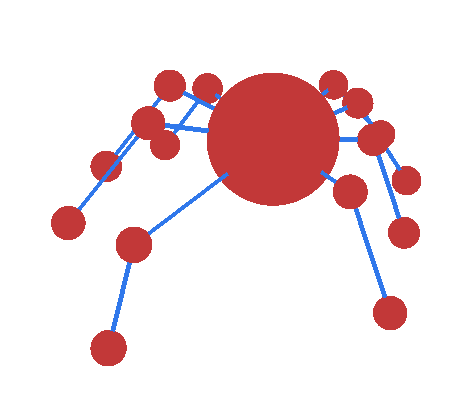
\includegraphics[width=\textwidth]{images/pavuk_kostra.png}
                \caption{Original spider input skeleton.}
                \label{fig:pavuk_skl_1}
        \end{subfigure}%
        ~ %add desired spacing between images, e. g. ~, \quad, \qquad etc.
          %(or a blank line to force the subfigure onto a new line)
        \begin{subfigure}[b]{0.4\textwidth}
        	\centering
                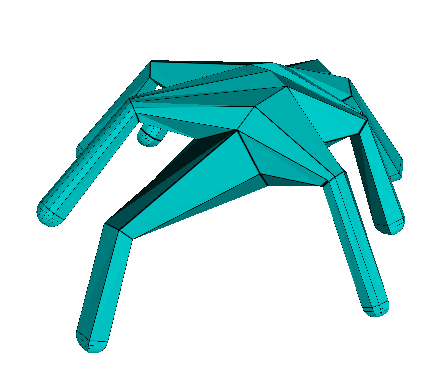
\includegraphics[width=\textwidth]{images/pavuk_fail.png}
                \caption{Base mesh from original skeleton with undesired mesh topology.}
                \label{fig:pavuk_mesh_1}
        \end{subfigure}
        \\ %add desired spacing between images, e. g. ~, \quad, \qquad etc.
          %(or a blank line to force the subfigure onto a new line)
        \begin{subfigure}[b]{0.4\textwidth}
        	\centering
                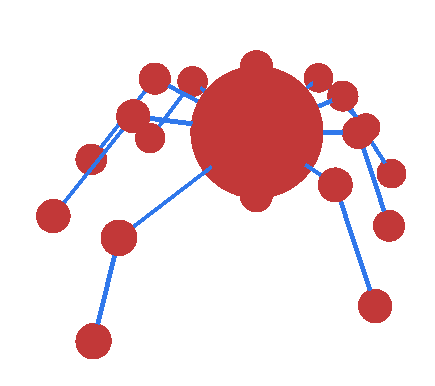
\includegraphics[width=\textwidth]{images/pavuk_kostra_upravena.png}
                \caption{Changed input skeleton to allow better triangulation.}
                \label{fig:pavuk_skl_2}
        \end{subfigure}
        ~ %add desired spacing between images, e. g. ~, \quad, \qquad etc.
          %(or a blank line to force the subfigure onto a new line)
        \begin{subfigure}[b]{0.4\textwidth}
        	\centering
                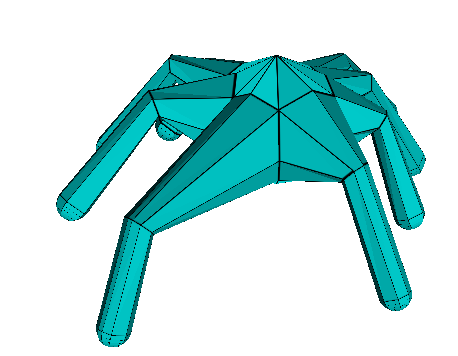
\includegraphics[width=\textwidth]{images/pavuk_dobry.png}
                \caption{Final base mesh with extra triangular faces but acceptable mesh topology.}
                \label{fig:pavuk_mesh_2}
        \end{subfigure}
        \caption[Base mesh of a spider]{Base mesh of a spider.}\label{fig:pavuk}
\end{figure}

\begin{figure}
    \centering
    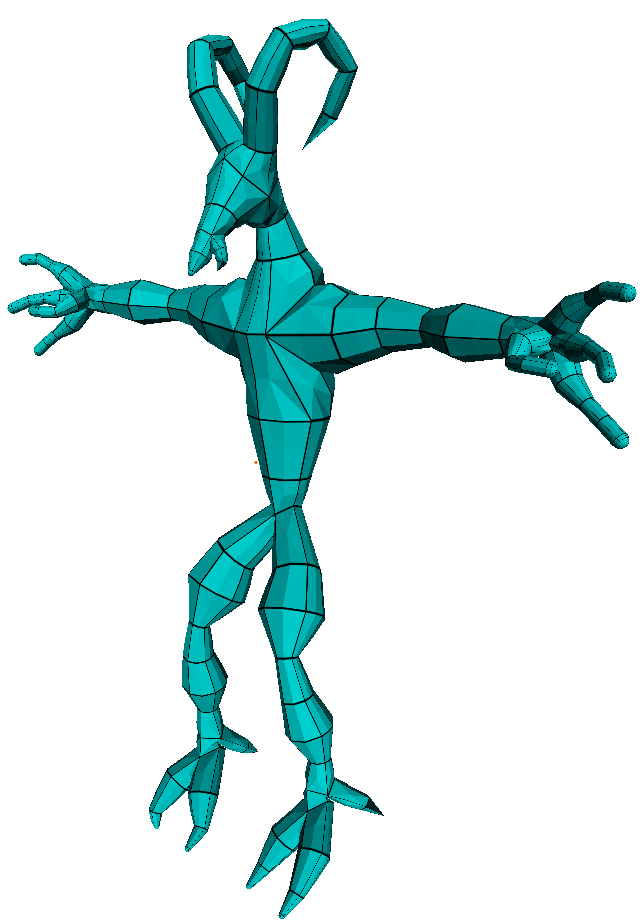
\includegraphics[width=\textwidth]{images/goat_1.png}
    \caption[Generated goat creature]{Goat creature generated with our algorithm. The input skeleton has 150 nodes. The node distribution is 9 branch nodes, 123 connection nodes, and 18 leaf nodes. Generated mesh consists of 1061 vertices, and 1126 faces. The mesh was generated in 0.074 s. The displayed mesh is tessellated with tessellation factor 2.}
    \label{fig:result_goat}
\end{figure}

\section{Linear and cyclic skeletons}

Linear and cyclic skeleton base mesh generation was introduced in this thesis.
Base meshes from linear skeletons without branching produce expected results.
Meshes produced by our algorithm have good edge flow and produce triangular faces only at the begging and end of the generated mesh.
The additional parameter setting the number of vertices for each node of a linear skeleton does not decrease the robustness of our approach.
Because with tessellation it is negligible.
A linear skeleton is shown in Figure \ref{fig:lin_skl} and generated base mesh in Figure \ref{fig:lin_mesh}.
In fact, with tessellation the mesh can be generated faster with the minimal number of vertices and still produce visual results equivalent to more complex meshes.
Generation of base meshes from cyclic skeletons produces good results.
The cycle can be at arbitrary place in the input skeleton.
Base meshes with various genuses can be generated.
However, the faces bridging cyclic nodes are formed solely by triangles.
This is caused by the fact that the valence of both one rings is not always equal.
Some of the triangular faces could be merged into quadrilaterals in a post-process similar to the one used in B-Mesh \cite{ji_bm}.
A cyclic input skeleton is shown in Figure \ref{fig:cyclic_skl} and its corresponding base mesh generated by our algorithm in Figure \ref{fig:cyclic_mesh}.

\begin{figure}[h]
        \centering
        \begin{subfigure}[b]{0.4\textwidth}
        	\centering
                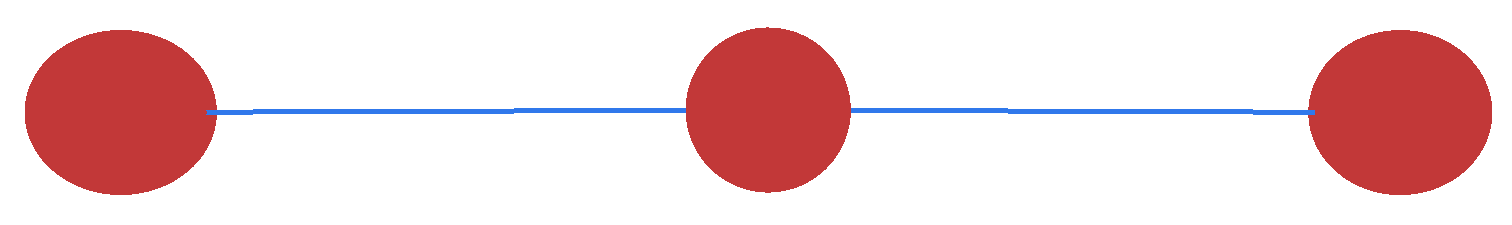
\includegraphics[width=\textwidth]{images/cerv_skl.png}
                \caption{Linear skeleton.}
                \label{fig:lin_skl}
        \end{subfigure}%
        \qquad %add desired spacing between images, e. g. ~, \quad, \qquad etc.
          %(or a blank line to force the subfigure onto a new line)
        \begin{subfigure}[b]{0.4\textwidth}
        	\centering
                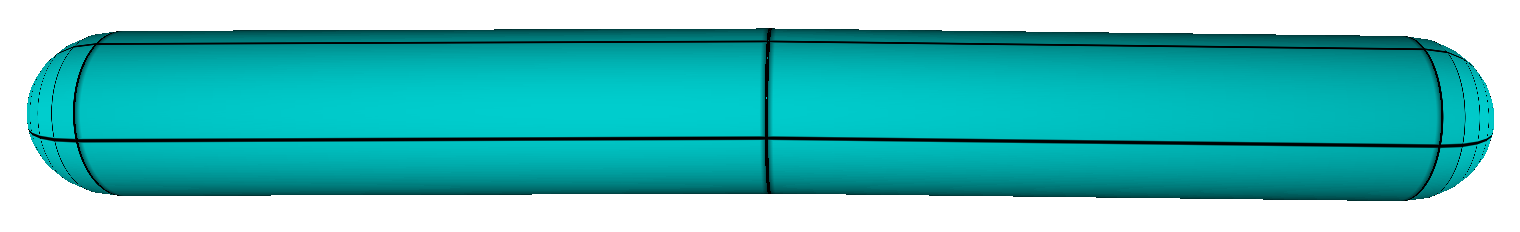
\includegraphics[width=\textwidth]{images/cerv_mesh.png}
                \caption{Tessellated linear base mesh.}
                \label{fig:lin_mesh}
        \end{subfigure}%
        \\ %add desired spacing between images, e. g. ~, \quad, \qquad etc.
          %(or a blank line to force the subfigure onto a new line)
        \begin{subfigure}[b]{0.5\textwidth}
        	\centering
                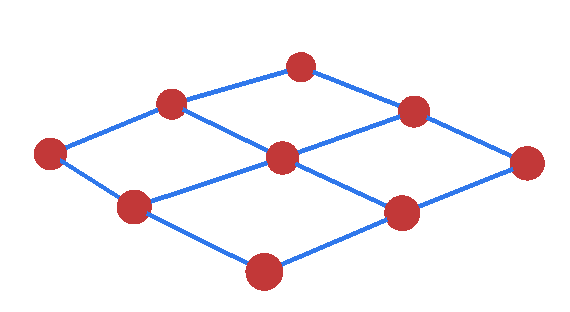
\includegraphics[width=\textwidth]{images/cycle_skl.png}
                \caption{Cyclic skeleton.}
                \label{fig:cyclic_skl}
        \end{subfigure}%
        ~ %add desired spacing between images, e. g. ~, \quad, \qquad etc.
          %(or a blank line to force the subfigure onto a new line)
        \begin{subfigure}[b]{0.5\textwidth}
        	\centering
                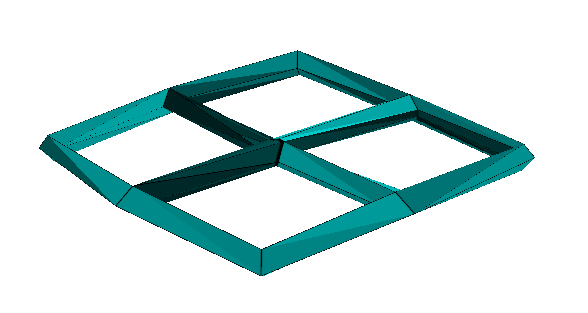
\includegraphics[width=\textwidth]{images/cycle_mesh.png}
                \caption{Base mesh with genus four.}
                \label{fig:cyclic_mesh}
        \end{subfigure}
        \caption[Cyclic and linear base meshes]{Cyclic and linear base meshes.}\label{fig:pavuk}
\end{figure}

\section{Capsules, ellipsoid nodes, and tessellation}

Capsules are automatically generated at leaf nodes.
The generated capsules can be naturally tessellated with our existing pipeline.
The number of nodes inserted into the input skeleton to form a capsule is currently automatically computed from the radius of a capsule node.
The automatic approach produces visually plausible capsules, especially when the generated base mesh is tessellated.
A capsule is shown in Figure \ref{fig:caps}.

Ellipsoid nodes can be defined as connection or branch nodes.
The generation of ellipsoid capsules is not yet supported.
Generated ellipsoids approximate the volume of the input skeleton.
Ellipsoid nodes can also be used to smooth sharp angles between two skeletal bones.
A slightly rotated sphere can produce better edge flow.
Ellipsoid nodes were used to generate fish in Figure \ref{fig:fish}.

Tessellation is used to increase the visual quality of generated base mesh in real time on GPU.
After tessellation the generated base mesh closely approximates the input skeleton.
However, the tessellated mesh can self-intersect.
This is mainly caused by the original input skeleton.
We attempted to solve this automatically without forcing the artist to edit the input skeleton by introducing radius scaling reduction.
Our radius scaling method helped with various self-intersecting meshes.
But certain meshes were still preferable to edit manually.
Generated base mesh is shown in Figure \ref{fig:no_tess}.
After tessellation the base mesh is shown in Figure \ref{fig:tess}.

\begin{figure}[h]
        \centering
        \begin{subfigure}[b]{0.25\textwidth}
        	\centering
                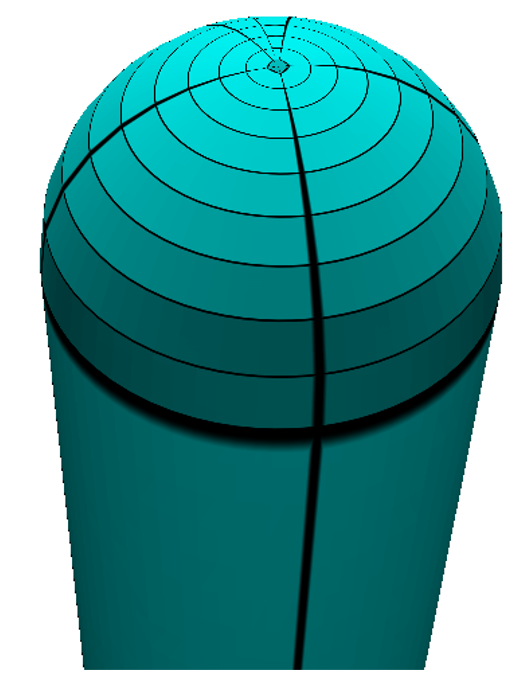
\includegraphics[height=\textwidth]{images/capsule.png}
                \caption{Leaf node capsule.}
                \label{fig:caps}
        \end{subfigure}%
        \qquad %add desired spacing between images, e. g. ~, \quad, \qquad etc.
          %(or a blank line to force the subfigure onto a new line)
        \begin{subfigure}[b]{0.4\textwidth}
        	\centering
                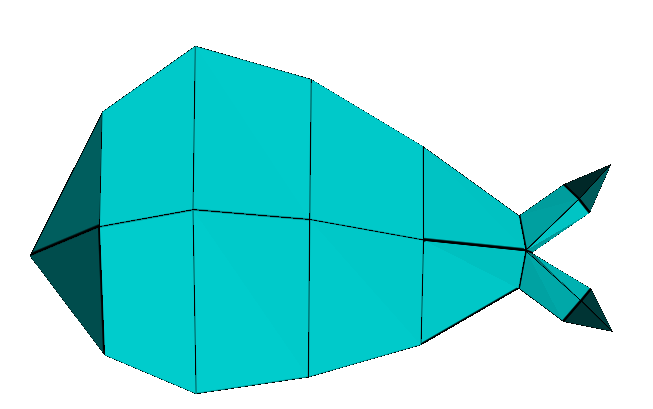
\includegraphics[width=\textwidth]{images/ryba_mesh.png}
                \caption{Fish with ellipsoid nodes.}
                \label{fig:fish}
        \end{subfigure}
        \caption[Capsules and ellipsoid nodes]{Capsules and ellipsoid nodes.}\label{fig:caps_ell}
\end{figure}

\begin{figure}[h]
        \centering
        \begin{subfigure}[b]{0.4\textwidth}
        	\centering
                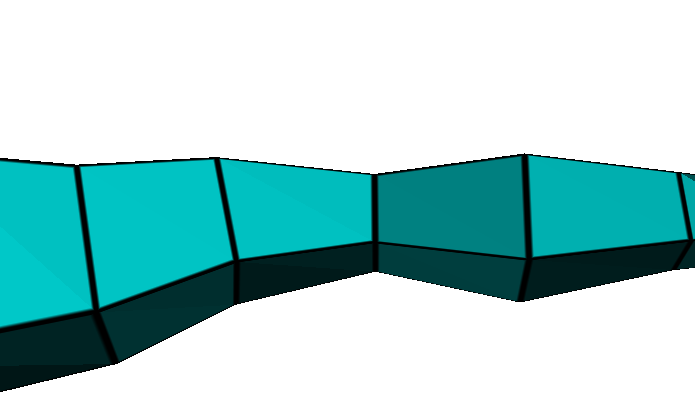
\includegraphics[width=0.8\textwidth]{images/not_tessellated_mesh.png}
                \caption{Non-tessellated mesh.}
                \label{fig:no_tess}
        \end{subfigure}
        \qquad %add desired spacing between images, e. g. ~, \quad, \qquad etc.
          %(or a blank line to force the subfigure onto a new line)
        \begin{subfigure}[b]{0.4\textwidth}
        	\centering
                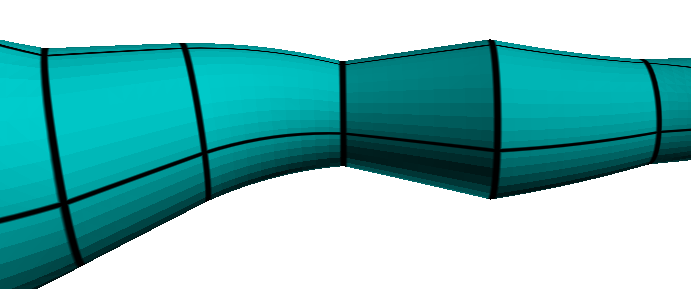
\includegraphics[width=0.8\textwidth]{images/tessellated_mesh.png}
                \caption{Tessellated mesh.}
                \label{fig:tess}
        \end{subfigure}
        \caption[Tessellation results]{Tessellation results.}\label{fig:tes_notess}
\end{figure}

\section{Comparison with SQM algorithm}

Our algorithm is also capable of generating base meshes from skeletons on which SQM would fail.
For example in Figure \ref{fig:comp_eel} we can see a fish as would be produced by SQM without ellipsoid nodes.
The generated base mesh resembles an eel.
Our algorithm with ellipsoid nodes Figure \ref{fig:comp_fish} produces a base mesh that corresponds to a fish.
In Figure \ref{fig:comp_cycle} we can see a cyclic mesh generated by our algorithm.
Producing a similar mesh in SQM is not possible as the cycles do not lie in symmetrical region of the input skeleton and SQM would not close them.
Figure \ref{fig:comp_cycle_sqm} shows base mesh from asymmetric cyclic skeleton as would be generated by SQM.

\begin{figure}[ht]
        \centering
        \begin{subfigure}[b]{0.45\textwidth}
        	\centering
			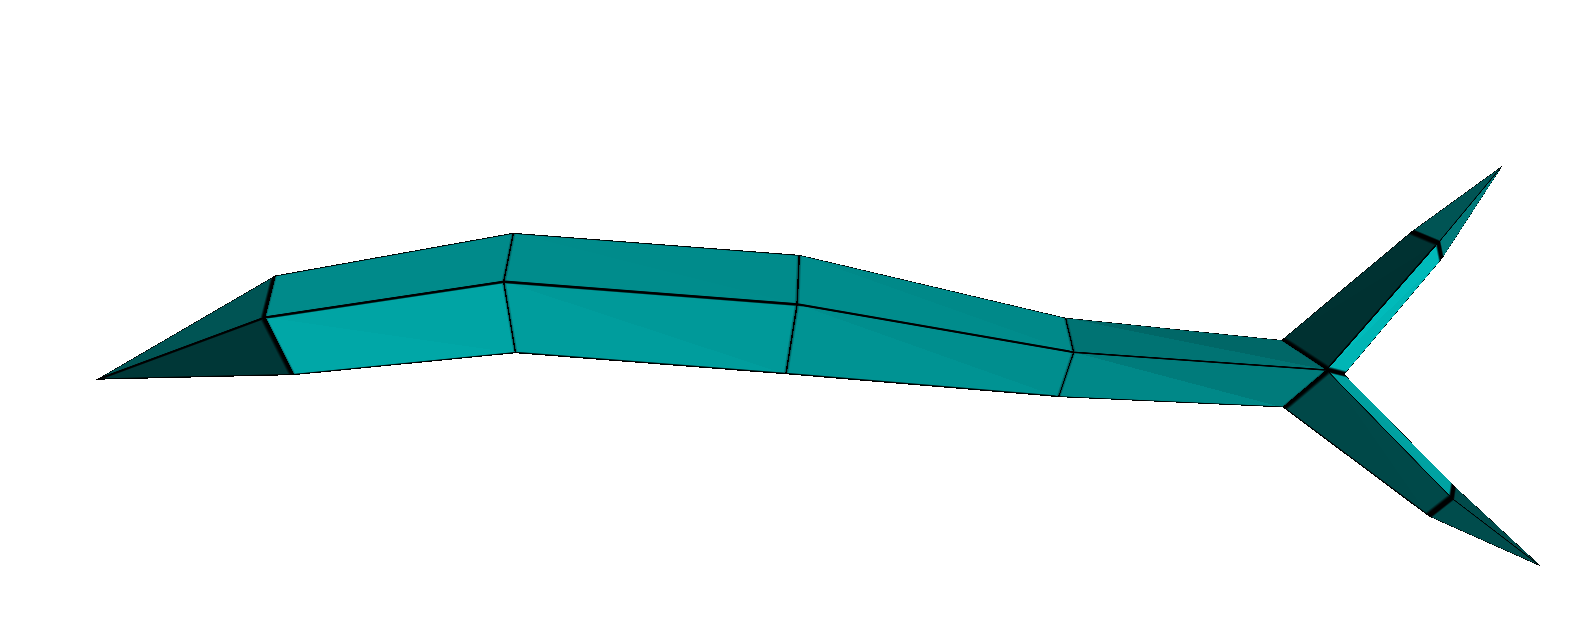
\includegraphics[width=0.8\textwidth]{images/ryba_no_elips}
            \caption{Fish without ellipsoid nodes as would be generated by SQM.}
            \label{fig:comp_eel}
        \end{subfigure}%
        ~ %add desired spacing between images, e. g. ~, \quad, \qquad etc.
          %(or a blank line to force the subfigure onto a new line)
        \begin{subfigure}[b]{0.45\textwidth}
        	\centering
			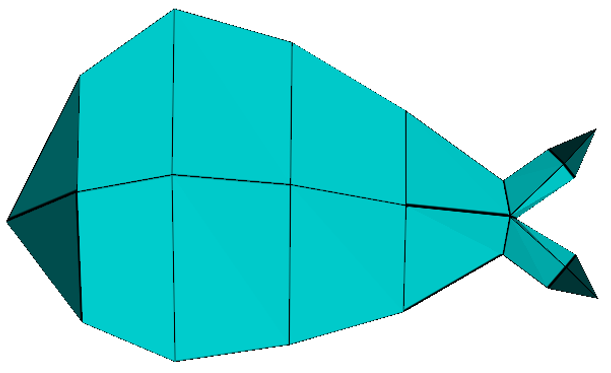
\includegraphics[width=0.7\textwidth]{images/ellipsoid_fish_ilu_2}
            \caption{Fish with ellipsoid nodes generated by our algorithm.}
            \label{fig:comp_fish}
        \end{subfigure}
        \\ %add desired spacing between images, e. g. ~, \quad, \qquad etc.
          %(or a blank line to force the subfigure onto a new line)
        \begin{subfigure}[b]{0.45\textwidth}
        	\centering
			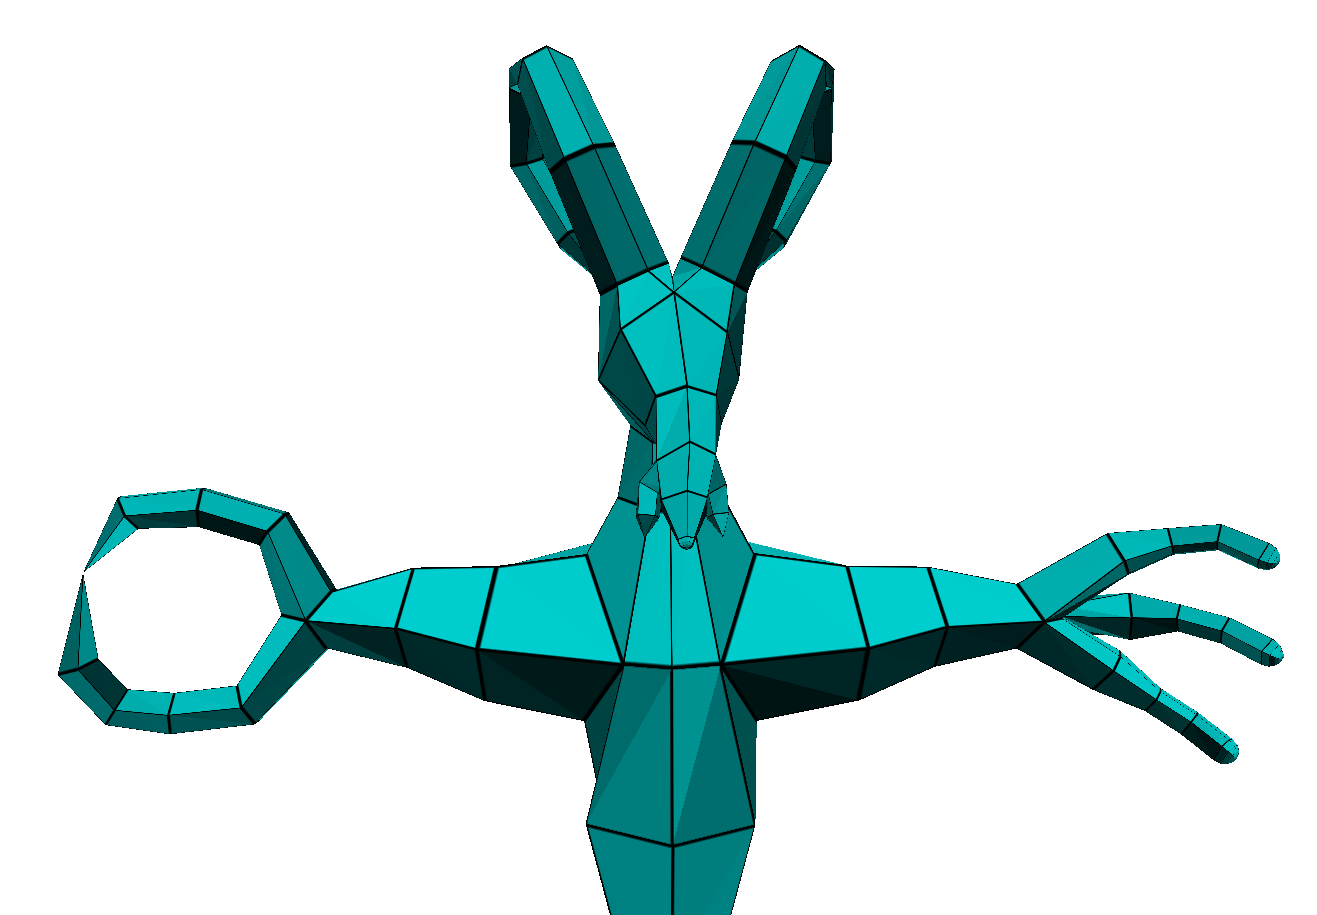
\includegraphics[width=0.9\textwidth]{images/goat_amput_sqm_3}
            \caption{Mesh from cyclic skeleton as would be generated by SQM.}
            \label{fig:comp_cycle_sqm}
        \end{subfigure}
        ~ %add desired spacing between images, e. g. ~, \quad, \qquad etc.
          %(or a blank line to force the subfigure onto a new line)
        \begin{subfigure}[b]{0.45\textwidth}
        	\centering
			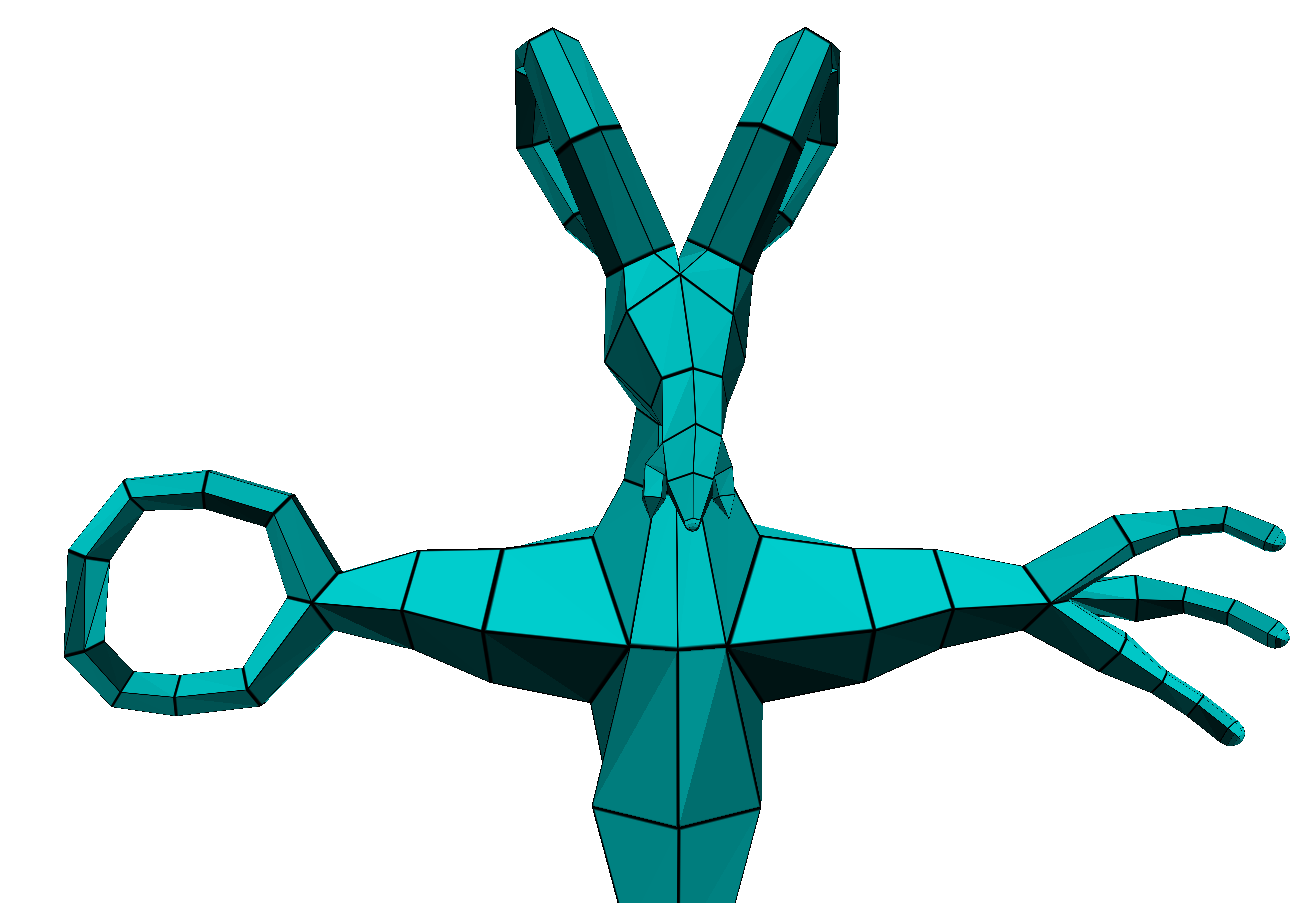
\includegraphics[width=0.9\textwidth]{images/goat_amput_3}
            \caption{Mesh from cyclic skeleton generated by our algorithm.}
            \label{fig:comp_cycle}
        \end{subfigure}
        \caption{Comparision of SQM (left) to our implementation (right).}
        \label{fig:comp_ilu}
\end{figure}

\section{Computation time}

In Table \ref{tab:models} we show the details about measured models.
For each model its total number of nodes as well as node distribution is shown.
Table \ref{tab:results} shows how much time each stage of our base manifold mesh algorithm takes.
Time was measured on Intel\textsuperscript{\textregistered}  Core\textsuperscript{TM} i7-3615QM a four core processor with each core clocked at 2.3 GHz.
Time is measured in milliseconds.
From the table we can see that the joining step, during which the tubular structure is generated, took the most time.
Therefore, it is a candidate for optimization since other steps of the algorithm took nearly no time to execute.
However, even at current speed we can generate base meshes at interactive frame rate.
For example, the goat creature shown in Figure \ref{fig:result_goat} can be generated 13.5 times per second.
From the tables we can also conclude that computation time is also highly dependent on the number of branch nodes and their number of neighbors.
For example, a dummy consisting of 140 nodes is computed in 57 milliseconds.
On the other hand a goat creature with 150 nodes is computed in 74 milliseconds.

BNP generation and subdivision steps are dependent on the number of branch nodes and number of neighbors of each branch node.
The more neighbors a node has the longer it takes to execute the triangulation.
The BNP joining step is limited by our used data structure.

%At each step of the algorithm the only prerequisite is that the parent of current node has been processed.
%We can exploit this fact and compute each child of a branch node in a parallel thread in order to increase the overall computation speed.
%If we want to increase the speed of computation with parallel joining of nodes we would need a half-edge data structure supporting parallel addition of vertices and edges.

\begin{table}[h]
\centering
\begin{tabular}{l|ccc||c}\hline
\multicolumn{1}{c}{\textbf{Model}} & \multicolumn{4}{c}{\textbf{Node Distribution}} \\
   & \#branch & \#connection & \#leaf & \textbf{\#nodes} \\ \hline
  worm & 21 & 2 & 0 & 23 \\
  dummy & 2 & 49 & 5 & 56 \\
  cycle & 1 & 12 & 1 & 14 \\
  octopus & 1 & 117 & 13 & 131 \\
  dummy 2 & 5 & 122 & 13 & 140 \\
  goat & 9 & 123 & 18 & 150 \\
  tree & 18 & 129 & 24 & 171 \\ \hline
\end{tabular}
\caption[Table show statics of input skeletons]{Table show statics of input skeletons. From left to right: name of the model, number of branch nodes, number of connection nodes, number of leaf nodes, and total number of nodes.}
\label{tab:models}
\end{table}

\begin{table}[h]
\centering
\begin{tabular}{l|cccc||c}\hline
\multicolumn{1}{c}{\textbf{Model}} & \multicolumn{5}{c}{\textbf{Timing of steps in computer clicks}} \\
   & straightening & generation & subdivision & joining & \textbf{Total} \\ \hline
  worm & 0 & 0 & 0 & 5 & 5 \\
  dummy & 0 & 4 & 2 & 15 & 21 \\
  cycle & 0 & 4 & 2 & 18 & 24 \\
  octopus & 1 & 9 & 5 & 54 & 69 \\
  dummy 2 & 1 & 11 & 6 & 39 & 57 \\
  goat & 1 & 16 & 10 & 47 & 74 \\
  tree & 3 & 28 & 15 & 50 & 96 \\ \hline
\end{tabular}
\caption[Table show statics of base mesh algorithm]{Table show statics of base mesh algorithm. From left to right: name of the model, timing of each step of the algorithm measured in milliseconds.}
\label{tab:results}
\end{table}



\appendix
\chapter{\TeX}

\LaTeX, \TeX



\newpage% or \cleardoublepage
% \pdfbookmark[<level>]{<title>}{<dest>}
\pdfbookmark[0]{Bibliography}{toc}
\bibliographystyle{plain} %cisla
%\bibliographystyle{alpha} %autor+rok
\bibliography{bibliography}


\end{document}
